\documentclass[1p]{elsarticle_modified}
%\bibliographystyle{elsarticle-num}

%\usepackage[colorlinks]{hyperref}
%\usepackage{abbrmath_seonhwa} %\Abb, \Ascr, \Acal ,\Abf, \Afrak
\usepackage{amsfonts}
\usepackage{amssymb}
\usepackage{amsmath}
\usepackage{amsthm}
\usepackage{scalefnt}
\usepackage{amsbsy}
\usepackage{kotex}
\usepackage{caption}
\usepackage{subfig}
\usepackage{color}
\usepackage{graphicx}
\usepackage{xcolor} %% white, black, red, green, blue, cyan, magenta, yellow
\usepackage{float}
\usepackage{setspace}
\usepackage{hyperref}

\usepackage{tikz}
\usetikzlibrary{arrows}

\usepackage{multirow}
\usepackage{array} % fixed length table
\usepackage{hhline}

%%%%%%%%%%%%%%%%%%%%%
\makeatletter
\renewcommand*\env@matrix[1][\arraystretch]{%
	\edef\arraystretch{#1}%
	\hskip -\arraycolsep
	\let\@ifnextchar\new@ifnextchar
	\array{*\c@MaxMatrixCols c}}
\makeatother %https://tex.stackexchange.com/questions/14071/how-can-i-increase-the-line-spacing-in-a-matrix
%%%%%%%%%%%%%%%

\usepackage[normalem]{ulem}

\newcommand{\msout}[1]{\ifmmode\text{\sout{\ensuremath{#1}}}\else\sout{#1}\fi}
%SOURCE: \msout is \stkout macro in https://tex.stackexchange.com/questions/20609/strikeout-in-math-mode

\newcommand{\cancel}[1]{
	\ifmmode
	{\color{red}\msout{#1}}
	\else
	{\color{red}\sout{#1}}
	\fi
}

\newcommand{\add}[1]{
	{\color{blue}\uwave{#1}}
}

\newcommand{\replace}[2]{
	\ifmmode
	{\color{red}\msout{#1}}{\color{blue}\uwave{#2}}
	\else
	{\color{red}\sout{#1}}{\color{blue}\uwave{#2}}
	\fi
}

\newcommand{\Sol}{\mathcal{S}} %segment
\newcommand{\D}{D} %diagram
\newcommand{\A}{\mathcal{A}} %arc


%%%%%%%%%%%%%%%%%%%%%%%%%%%%%5 test

\def\sl{\operatorname{\textup{SL}}(2,\Cbb)}
\def\psl{\operatorname{\textup{PSL}}(2,\Cbb)}
\def\quan{\mkern 1mu \triangleright \mkern 1mu}

\theoremstyle{definition}
\newtheorem{thm}{Theorem}[section]
\newtheorem{prop}[thm]{Proposition}
\newtheorem{lem}[thm]{Lemma}
\newtheorem{ques}[thm]{Question}
\newtheorem{cor}[thm]{Corollary}
\newtheorem{defn}[thm]{Definition}
\newtheorem{exam}[thm]{Example}
\newtheorem{rmk}[thm]{Remark}
\newtheorem{alg}[thm]{Algorithm}

\newcommand{\I}{\sqrt{-1}}
\begin{document}

%\begin{frontmatter}
%
%\title{Boundary parabolic representations of knots up to 8 crossings}
%
%%% Group authors per affiliation:
%\author{Yunhi Cho} 
%\address{Department of Mathematics, University of Seoul, Seoul, Korea}
%\ead{yhcho@uos.ac.kr}
%
%
%\author{Seonhwa Kim} %\fnref{s_kim}}
%\address{Center for Geometry and Physics, Institute for Basic Science, Pohang, 37673, Korea}
%\ead{ryeona17@ibs.re.kr}
%
%\author{Hyuk Kim}
%\address{Department of Mathematical Sciences, Seoul National University, Seoul 08826, Korea}
%\ead{hyukkim@snu.ac.kr}
%
%\author{Seokbeom Yoon}
%\address{Department of Mathematical Sciences, Seoul National University, Seoul, 08826,  Korea}
%\ead{sbyoon15@snu.ac.kr}
%
%\begin{abstract}
%We find all boundary parabolic representation of knots up to 8 crossings.
%
%\end{abstract}
%\begin{keyword}
%    \MSC[2010] 57M25 
%\end{keyword}
%
%\end{frontmatter}

%\linenumbers
%\tableofcontents
%
\newcommand\colored[1]{\textcolor{white}{\rule[-0.35ex]{0.8em}{1.4ex}}\kern-0.8em\color{red} #1}%
%\newcommand\colored[1]{\textcolor{white}{ #1}\kern-2.17ex	\textcolor{white}{ #1}\kern-1.81ex	\textcolor{white}{ #1}\kern-2.15ex\color{red}#1	}

{\Large $\underline{12a_{0431}~(K12a_{0431})}$}

\setlength{\tabcolsep}{10pt}
\renewcommand{\arraystretch}{1.6}
\vspace{1cm}\begin{tabular}{m{100pt}>{\centering\arraybackslash}m{274pt}}
\multirow{5}{120pt}{
	\centering
	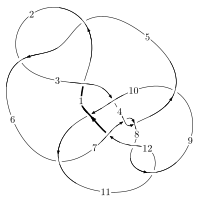
\includegraphics[width=112pt]{../../../GIT/diagram.site/Diagrams/png/1232_12a_0431.png}\\
\ \ \ A knot diagram\footnotemark}&
\allowdisplaybreaks
\textbf{Linearized knot diagam} \\
\cline{2-2}
 &
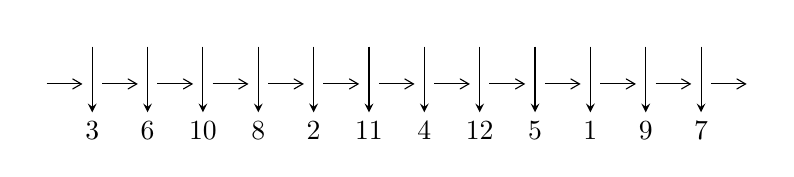
\begin{tikzpicture}[x=20pt, y=17pt]
	% nodes
	\node (C0) at (0, 0) {};
	\node (C1) at (1, 0) {};
	\node (C1U) at (1, +1) {};
	\node (C1D) at (1, -1) {3};

	\node (C2) at (2, 0) {};
	\node (C2U) at (2, +1) {};
	\node (C2D) at (2, -1) {6};

	\node (C3) at (3, 0) {};
	\node (C3U) at (3, +1) {};
	\node (C3D) at (3, -1) {10};

	\node (C4) at (4, 0) {};
	\node (C4U) at (4, +1) {};
	\node (C4D) at (4, -1) {8};

	\node (C5) at (5, 0) {};
	\node (C5U) at (5, +1) {};
	\node (C5D) at (5, -1) {2};

	\node (C6) at (6, 0) {};
	\node (C6U) at (6, +1) {};
	\node (C6D) at (6, -1) {11};

	\node (C7) at (7, 0) {};
	\node (C7U) at (7, +1) {};
	\node (C7D) at (7, -1) {4};

	\node (C8) at (8, 0) {};
	\node (C8U) at (8, +1) {};
	\node (C8D) at (8, -1) {12};

	\node (C9) at (9, 0) {};
	\node (C9U) at (9, +1) {};
	\node (C9D) at (9, -1) {5};

	\node (C10) at (10, 0) {};
	\node (C10U) at (10, +1) {};
	\node (C10D) at (10, -1) {1};

	\node (C11) at (11, 0) {};
	\node (C11U) at (11, +1) {};
	\node (C11D) at (11, -1) {9};

	\node (C12) at (12, 0) {};
	\node (C12U) at (12, +1) {};
	\node (C12D) at (12, -1) {7};
	\node (C13) at (13, 0) {};

	% arrows
	\draw[->,>={angle 60}]
	(C0) edge (C1) (C1) edge (C2) (C2) edge (C3) (C3) edge (C4) (C4) edge (C5) (C5) edge (C6) (C6) edge (C7) (C7) edge (C8) (C8) edge (C9) (C9) edge (C10) (C10) edge (C11) (C11) edge (C12) (C12) edge (C13) ;	\draw[->,>=stealth]
	(C1U) edge (C1D) (C2U) edge (C2D) (C3U) edge (C3D) (C4U) edge (C4D) (C5U) edge (C5D) (C6U) edge (C6D) (C7U) edge (C7D) (C8U) edge (C8D) (C9U) edge (C9D) (C10U) edge (C10D) (C11U) edge (C11D) (C12U) edge (C12D) ;
	\end{tikzpicture} \\
\hhline{~~} \\& 
\textbf{Solving Sequence} \\ \cline{2-2} 
 &
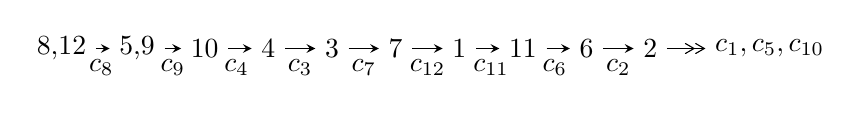
\begin{tikzpicture}[x=23pt, y=7pt]
	% node
	\node (A0) at (-1/8, 0) {8,12};
	\node (A1) at (17/16, 0) {5,9};
	\node (A2) at (17/8, 0) {10};
	\node (A3) at (25/8, 0) {4};
	\node (A4) at (33/8, 0) {3};
	\node (A5) at (41/8, 0) {7};
	\node (A6) at (49/8, 0) {1};
	\node (A7) at (57/8, 0) {11};
	\node (A8) at (65/8, 0) {6};
	\node (A9) at (73/8, 0) {2};
	\node (C1) at (1/2, -1) {$c_{8}$};
	\node (C2) at (13/8, -1) {$c_{9}$};
	\node (C3) at (21/8, -1) {$c_{4}$};
	\node (C4) at (29/8, -1) {$c_{3}$};
	\node (C5) at (37/8, -1) {$c_{7}$};
	\node (C6) at (45/8, -1) {$c_{12}$};
	\node (C7) at (53/8, -1) {$c_{11}$};
	\node (C8) at (61/8, -1) {$c_{6}$};
	\node (C9) at (69/8, -1) {$c_{2}$};
	\node (A10) at (11, 0) {$c_{1},c_{5},c_{10}$};

	% edge
	\draw[->,>=stealth]	
	(A0) edge (A1) (A1) edge (A2) (A2) edge (A3) (A3) edge (A4) (A4) edge (A5) (A5) edge (A6) (A6) edge (A7) (A7) edge (A8) (A8) edge (A9) ;
	\draw[->>,>={angle 60}]	
	(A9) edge (A10);
\end{tikzpicture} \\ 

\end{tabular} \\

\footnotetext{
The image of knot diagram is generated by the software ``\textbf{Draw programme}" developed by Andrew Bartholomew(\url{http://www.layer8.co.uk/maths/draw/index.htm\#Running-draw}), where we modified some parts for our purpose(\url{https://github.com/CATsTAILs/LinksPainter}).
}\phantom \\ \newline 
\centering \textbf{Ideals for irreducible components\footnotemark of $X_{\text{par}}$} 
 
\begin{align*}
I^u_{1}&=\langle 
-1.08221\times10^{1017} u^{182}+1.35395\times10^{1018} u^{181}+\cdots+2.55657\times10^{1018} b+6.03949\times10^{1020},\\
\phantom{I^u_{1}}&\phantom{= \langle  }6.03054\times10^{1019} u^{182}-8.16888\times10^{1020} u^{181}+\cdots+2.10491\times10^{1020} a+2.67814\times10^{1023},\\
\phantom{I^u_{1}}&\phantom{= \langle  }u^{183}-13 u^{182}+\cdots+6260 u-3952\rangle \\
I^u_{2}&=\langle 
-5.30317\times10^{15} u^{45}+9.11536\times10^{16} u^{44}+\cdots+9.18144\times10^{14} b-6.45933\times10^{16},\\
\phantom{I^u_{2}}&\phantom{= \langle  }1.83232\times10^{17} u^{45}-3.25201\times10^{18} u^{44}+\cdots+6.42701\times10^{15} a+4.76357\times10^{17},\;u^{46}-18 u^{45}+\cdots-97 u+7\rangle \\
\\
\end{align*}
\raggedright * 2 irreducible components of $\dim_{\mathbb{C}}=0$, with total 229 representations.\\
\footnotetext{All coefficients of polynomials are rational numbers. But the coefficients are sometimes approximated in decimal forms when there is not enough margin.}
\newpage
\renewcommand{\arraystretch}{1}
\centering \section*{I. $I^u_{1}= \langle -1.08\times10^{1017} u^{182}+1.35\times10^{1018} u^{181}+\cdots+2.56\times10^{1018} b+6.04\times10^{1020},\;6.03\times10^{1019} u^{182}-8.17\times10^{1020} u^{181}+\cdots+2.10\times10^{1020} a+2.68\times10^{1023},\;u^{183}-13 u^{182}+\cdots+6260 u-3952 \rangle$}
\flushleft \textbf{(i) Arc colorings}\\
\begin{tabular}{m{7pt} m{180pt} m{7pt} m{180pt} }
\flushright $a_{8}=$&$\begin{pmatrix}1\\0\end{pmatrix}$ \\
\flushright $a_{12}=$&$\begin{pmatrix}0\\u\end{pmatrix}$ \\
\flushright $a_{5}=$&$\begin{pmatrix}-0.286499 u^{182}+3.88088 u^{181}+\cdots+4569.49 u-1272.33\\0.0423306 u^{182}-0.529598 u^{181}+\cdots+222.058 u-236.235\end{pmatrix}$ \\
\flushright $a_{9}=$&$\begin{pmatrix}1\\u^2\end{pmatrix}$ \\
\flushright $a_{10}=$&$\begin{pmatrix}0.387179 u^{182}-4.99816 u^{181}+\cdots-1287.11 u-949.545\\0.0501010 u^{182}-0.653556 u^{181}+\cdots-265.486 u-132.693\end{pmatrix}$ \\
\flushright $a_{4}=$&$\begin{pmatrix}-0.244169 u^{182}+3.35128 u^{181}+\cdots+4791.55 u-1508.57\\0.0423306 u^{182}-0.529598 u^{181}+\cdots+222.058 u-236.235\end{pmatrix}$ \\
\flushright $a_{3}=$&$\begin{pmatrix}-0.117373 u^{182}+1.35855 u^{181}+\cdots-1035.35 u+1306.01\\-0.111769 u^{182}+1.45629 u^{181}+\cdots+1217.32 u-0.425868\end{pmatrix}$ \\
\flushright $a_{7}=$&$\begin{pmatrix}-0.150852 u^{182}+1.98096 u^{181}+\cdots+1225.75 u+102.938\\0.00953673 u^{182}-0.157843 u^{181}+\cdots-704.908 u+345.154\end{pmatrix}$ \\
\flushright $a_{1}=$&$\begin{pmatrix}-0.119555 u^{182}+1.73225 u^{181}+\cdots+3788.50 u-1319.55\\-0.0310668 u^{182}+0.464528 u^{181}+\cdots+1509.59 u-561.843\end{pmatrix}$ \\
\flushright $a_{11}=$&$\begin{pmatrix}u\\u^3+u\end{pmatrix}$ \\
\flushright $a_{6}=$&$\begin{pmatrix}-0.193264 u^{182}+2.55272 u^{181}+\cdots+1827.85 u-18.6801\\-0.0164454 u^{182}+0.188229 u^{181}+\cdots-398.097 u+304.139\end{pmatrix}$ \\
\flushright $a_{2}=$&$\begin{pmatrix}0.0929241 u^{182}-1.36603 u^{181}+\cdots-2642.26 u+1101.99\\-0.0701137 u^{182}+0.884804 u^{181}+\cdots+214.247 u+298.614\end{pmatrix}$\\&\end{tabular}
\flushleft \textbf{(ii) Obstruction class $= -1$}\\~\\
\flushleft \textbf{(iii) Cusp Shapes $= -0.0678249 u^{182}+0.743225 u^{181}+\cdots-2271.57 u+1265.71$}\\~\\
\newpage\renewcommand{\arraystretch}{1}
\flushleft \textbf{(iv) u-Polynomials at the component}\newline \\
\begin{tabular}{m{50pt}|m{274pt}}
Crossings & \hspace{64pt}u-Polynomials at each crossing \\
\hline $$\begin{aligned}c_{1}\end{aligned}$$&$\begin{aligned}
&u^{183}+82 u^{182}+\cdots+16 u+1
\end{aligned}$\\
\hline $$\begin{aligned}c_{2},c_{5}\end{aligned}$$&$\begin{aligned}
&u^{183}+4 u^{182}+\cdots+20 u+1
\end{aligned}$\\
\hline $$\begin{aligned}c_{3}\end{aligned}$$&$\begin{aligned}
&u^{183}+2 u^{182}+\cdots+136040 u+44287
\end{aligned}$\\
\hline $$\begin{aligned}c_{4},c_{7}\end{aligned}$$&$\begin{aligned}
&u^{183}+2 u^{182}+\cdots+30967 u+8921
\end{aligned}$\\
\hline $$\begin{aligned}c_{6}\end{aligned}$$&$\begin{aligned}
&u^{183}-2 u^{182}+\cdots+10862 u+527
\end{aligned}$\\
\hline $$\begin{aligned}c_{8},c_{11}\end{aligned}$$&$\begin{aligned}
&u^{183}+13 u^{182}+\cdots+6260 u+3952
\end{aligned}$\\
\hline $$\begin{aligned}c_{9}\end{aligned}$$&$\begin{aligned}
&u^{183}- u^{182}+\cdots+36530383 u+15439309
\end{aligned}$\\
\hline $$\begin{aligned}c_{10}\end{aligned}$$&$\begin{aligned}
&u^{183}-13 u^{182}+\cdots+808 u+1
\end{aligned}$\\
\hline $$\begin{aligned}c_{12}\end{aligned}$$&$\begin{aligned}
&u^{183}+8 u^{182}+\cdots-9354518 u+728723
\end{aligned}$\\
\hline
\end{tabular}\\~\\
\newpage\renewcommand{\arraystretch}{1}
\flushleft \textbf{(v) Riley Polynomials at the component}\newline \\
\begin{tabular}{m{50pt}|m{274pt}}
Crossings & \hspace{64pt}Riley Polynomials at each crossing \\
\hline $$\begin{aligned}c_{1}\end{aligned}$$&$\begin{aligned}
&y^{183}+50 y^{182}+\cdots+4624 y-1
\end{aligned}$\\
\hline $$\begin{aligned}c_{2},c_{5}\end{aligned}$$&$\begin{aligned}
&y^{183}-82 y^{182}+\cdots+16 y-1
\end{aligned}$\\
\hline $$\begin{aligned}c_{3}\end{aligned}$$&$\begin{aligned}
&y^{183}+4 y^{182}+\cdots-261117339144 y-1961338369
\end{aligned}$\\
\hline $$\begin{aligned}c_{4},c_{7}\end{aligned}$$&$\begin{aligned}
&y^{183}-100 y^{182}+\cdots+3828341213 y-79584241
\end{aligned}$\\
\hline $$\begin{aligned}c_{6}\end{aligned}$$&$\begin{aligned}
&y^{183}+26 y^{182}+\cdots-28715838 y-277729
\end{aligned}$\\
\hline $$\begin{aligned}c_{8},c_{11}\end{aligned}$$&$\begin{aligned}
&y^{183}+99 y^{182}+\cdots-447121808 y-15618304
\end{aligned}$\\
\hline $$\begin{aligned}c_{9}\end{aligned}$$&$\begin{aligned}
&y^{183}- y^{182}+\cdots+6862895901260619 y-238372262397481
\end{aligned}$\\
\hline $$\begin{aligned}c_{10}\end{aligned}$$&$\begin{aligned}
&y^{183}+15 y^{182}+\cdots+315098 y-1
\end{aligned}$\\
\hline $$\begin{aligned}c_{12}\end{aligned}$$&$\begin{aligned}
&y^{183}+2 y^{182}+\cdots-44241446103030 y-531037210729
\end{aligned}$\\
\hline
\end{tabular}\\~\\
\newpage\flushleft \textbf{(vi) Complex Volumes and Cusp Shapes}
$$\begin{array}{c|c|c}  
\text{Solutions to }I^u_{1}& \I (\text{vol} + \sqrt{-1}CS) & \text{Cusp shape}\\
 \hline 
\begin{aligned}
u &= \phantom{-}0.109145 + 1.004260 I \\
a &= -0.32645 + 1.94373 I \\
b &= \phantom{-}0.46884 - 1.59401 I\end{aligned}
 & \phantom{-}5.73632 + 2.61032 I & \phantom{-0.000000 } 0 \\ \hline\begin{aligned}
u &= \phantom{-}0.109145 - 1.004260 I \\
a &= -0.32645 - 1.94373 I \\
b &= \phantom{-}0.46884 + 1.59401 I\end{aligned}
 & \phantom{-}5.73632 - 2.61032 I & \phantom{-0.000000 } 0 \\ \hline\begin{aligned}
u &= \phantom{-}0.474605 + 0.855807 I \\
a &= -0.16105 - 1.96522 I \\
b &= \phantom{-}0.936293 + 0.779716 I\end{aligned}
 & -0.11444 - 4.46856 I & \phantom{-0.000000 } 0 \\ \hline\begin{aligned}
u &= \phantom{-}0.474605 - 0.855807 I \\
a &= -0.16105 + 1.96522 I \\
b &= \phantom{-}0.936293 - 0.779716 I\end{aligned}
 & -0.11444 + 4.46856 I & \phantom{-0.000000 } 0 \\ \hline\begin{aligned}
u &= \phantom{-}0.787313 + 0.573287 I \\
a &= -0.481590 + 0.075837 I \\
b &= -1.200510 - 0.275493 I\end{aligned}
 & -3.41227 - 6.64607 I & \phantom{-0.000000 } 0 \\ \hline\begin{aligned}
u &= \phantom{-}0.787313 - 0.573287 I \\
a &= -0.481590 - 0.075837 I \\
b &= -1.200510 + 0.275493 I\end{aligned}
 & -3.41227 + 6.64607 I & \phantom{-0.000000 } 0 \\ \hline\begin{aligned}
u &= -0.431412 + 0.951554 I \\
a &= \phantom{-}0.61887 - 1.92842 I \\
b &= -1.197510 + 0.388597 I\end{aligned}
 & -6.95643 + 2.58003 I & \phantom{-0.000000 } 0 \\ \hline\begin{aligned}
u &= -0.431412 - 0.951554 I \\
a &= \phantom{-}0.61887 + 1.92842 I \\
b &= -1.197510 - 0.388597 I\end{aligned}
 & -6.95643 - 2.58003 I & \phantom{-0.000000 } 0 \\ \hline\begin{aligned}
u &= -0.224766 + 0.923643 I \\
a &= \phantom{-}0.29247 + 1.45607 I \\
b &= \phantom{-}0.967832 - 0.499646 I\end{aligned}
 & \phantom{-}0.203430 + 0.797452 I & \phantom{-0.000000 } 0 \\ \hline\begin{aligned}
u &= -0.224766 - 0.923643 I \\
a &= \phantom{-}0.29247 - 1.45607 I \\
b &= \phantom{-}0.967832 + 0.499646 I\end{aligned}
 & \phantom{-}0.203430 - 0.797452 I & \phantom{-0.000000 } 0\\
 \hline 
 \end{array}$$\newpage$$\begin{array}{c|c|c}  
\text{Solutions to }I^u_{1}& \I (\text{vol} + \sqrt{-1}CS) & \text{Cusp shape}\\
 \hline 
\begin{aligned}
u &= -0.146019 + 1.045120 I \\
a &= -0.70016 - 1.67400 I \\
b &= \phantom{-}0.296606 + 1.315740 I\end{aligned}
 & \phantom{-}5.88429 - 2.90843 I & \phantom{-0.000000 } 0 \\ \hline\begin{aligned}
u &= -0.146019 - 1.045120 I \\
a &= -0.70016 + 1.67400 I \\
b &= \phantom{-}0.296606 - 1.315740 I\end{aligned}
 & \phantom{-}5.88429 + 2.90843 I & \phantom{-0.000000 } 0 \\ \hline\begin{aligned}
u &= \phantom{-}0.089576 + 1.061220 I \\
a &= -0.03862 - 1.84294 I \\
b &= -0.11882 + 1.47999 I\end{aligned}
 & \phantom{-}5.79090 - 3.15817 I & \phantom{-0.000000 } 0 \\ \hline\begin{aligned}
u &= \phantom{-}0.089576 - 1.061220 I \\
a &= -0.03862 + 1.84294 I \\
b &= -0.11882 - 1.47999 I\end{aligned}
 & \phantom{-}5.79090 + 3.15817 I & \phantom{-0.000000 } 0 \\ \hline\begin{aligned}
u &= -0.491782 + 0.787874 I \\
a &= \phantom{-}0.63547 - 1.75863 I \\
b &= -1.234790 + 0.402039 I\end{aligned}
 & -3.35915 - 5.35503 I & \phantom{-0.000000 } 0 \\ \hline\begin{aligned}
u &= -0.491782 - 0.787874 I \\
a &= \phantom{-}0.63547 + 1.75863 I \\
b &= -1.234790 - 0.402039 I\end{aligned}
 & -3.35915 + 5.35503 I & \phantom{-0.000000 } 0 \\ \hline\begin{aligned}
u &= -0.398828 + 0.831123 I \\
a &= \phantom{-}0.05013 - 1.70457 I \\
b &= -1.65689 + 0.06147 I\end{aligned}
 & -8.67420 + 1.70955 I & \phantom{-0.000000 } 0 \\ \hline\begin{aligned}
u &= -0.398828 - 0.831123 I \\
a &= \phantom{-}0.05013 + 1.70457 I \\
b &= -1.65689 - 0.06147 I\end{aligned}
 & -8.67420 - 1.70955 I & \phantom{-0.000000 } 0 \\ \hline\begin{aligned}
u &= \phantom{-}0.042485 + 0.916931 I \\
a &= -0.07239 + 2.04280 I \\
b &= \phantom{-}1.083850 - 0.608952 I\end{aligned}
 & \phantom{-}1.34148 + 3.84832 I & \phantom{-0.000000 } 0 \\ \hline\begin{aligned}
u &= \phantom{-}0.042485 - 0.916931 I \\
a &= -0.07239 - 2.04280 I \\
b &= \phantom{-}1.083850 + 0.608952 I\end{aligned}
 & \phantom{-}1.34148 - 3.84832 I & \phantom{-0.000000 } 0\\
 \hline 
 \end{array}$$\newpage$$\begin{array}{c|c|c}  
\text{Solutions to }I^u_{1}& \I (\text{vol} + \sqrt{-1}CS) & \text{Cusp shape}\\
 \hline 
\begin{aligned}
u &= \phantom{-}0.253570 + 1.056280 I \\
a &= \phantom{-}0.675074 + 0.822827 I \\
b &= -0.397454 - 0.735287 I\end{aligned}
 & \phantom{-}2.06637 - 1.14443 I & \phantom{-0.000000 } 0 \\ \hline\begin{aligned}
u &= \phantom{-}0.253570 - 1.056280 I \\
a &= \phantom{-}0.675074 - 0.822827 I \\
b &= -0.397454 + 0.735287 I\end{aligned}
 & \phantom{-}2.06637 + 1.14443 I & \phantom{-0.000000 } 0 \\ \hline\begin{aligned}
u &= -0.303028 + 1.053370 I \\
a &= -0.74779 + 2.44925 I \\
b &= \phantom{-}1.151140 - 0.297713 I\end{aligned}
 & \phantom{-}0.37592 + 4.43107 I & \phantom{-0.000000 } 0 \\ \hline\begin{aligned}
u &= -0.303028 - 1.053370 I \\
a &= -0.74779 - 2.44925 I \\
b &= \phantom{-}1.151140 + 0.297713 I\end{aligned}
 & \phantom{-}0.37592 - 4.43107 I & \phantom{-0.000000 } 0 \\ \hline\begin{aligned}
u &= -0.398687 + 0.798508 I \\
a &= -0.56518 + 1.73812 I \\
b &= \phantom{-}1.225740 - 0.381156 I\end{aligned}
 & -1.337870 + 0.050450 I & \phantom{-0.000000 } 0 \\ \hline\begin{aligned}
u &= -0.398687 - 0.798508 I \\
a &= -0.56518 - 1.73812 I \\
b &= \phantom{-}1.225740 + 0.381156 I\end{aligned}
 & -1.337870 - 0.050450 I & \phantom{-0.000000 } 0 \\ \hline\begin{aligned}
u &= \phantom{-}0.434704 + 1.025960 I \\
a &= -0.391022 + 1.152800 I \\
b &= \phantom{-}0.452956 - 0.741335 I\end{aligned}
 & -0.139475 - 0.478764 I & \phantom{-0.000000 } 0 \\ \hline\begin{aligned}
u &= \phantom{-}0.434704 - 1.025960 I \\
a &= -0.391022 - 1.152800 I \\
b &= \phantom{-}0.452956 + 0.741335 I\end{aligned}
 & -0.139475 + 0.478764 I & \phantom{-0.000000 } 0 \\ \hline\begin{aligned}
u &= -0.458957 + 0.752394 I \\
a &= \phantom{-}0.73148 + 1.43664 I \\
b &= \phantom{-}0.972081 - 0.615995 I\end{aligned}
 & \phantom{-}0.094435 + 0.634449 I & \phantom{-0.000000 } 0 \\ \hline\begin{aligned}
u &= -0.458957 - 0.752394 I \\
a &= \phantom{-}0.73148 - 1.43664 I \\
b &= \phantom{-}0.972081 + 0.615995 I\end{aligned}
 & \phantom{-}0.094435 - 0.634449 I & \phantom{-0.000000 } 0\\
 \hline 
 \end{array}$$\newpage$$\begin{array}{c|c|c}  
\text{Solutions to }I^u_{1}& \I (\text{vol} + \sqrt{-1}CS) & \text{Cusp shape}\\
 \hline 
\begin{aligned}
u &= \phantom{-}0.702531 + 0.872299 I \\
a &= \phantom{-}0.202738 - 0.517122 I \\
b &= -0.998318 + 0.365025 I\end{aligned}
 & -2.20573 - 4.10299 I & \phantom{-0.000000 } 0 \\ \hline\begin{aligned}
u &= \phantom{-}0.702531 - 0.872299 I \\
a &= \phantom{-}0.202738 + 0.517122 I \\
b &= -0.998318 - 0.365025 I\end{aligned}
 & -2.20573 + 4.10299 I & \phantom{-0.000000 } 0 \\ \hline\begin{aligned}
u &= \phantom{-}1.130090 + 0.012260 I \\
a &= -0.087064 - 0.118191 I \\
b &= -1.135540 - 0.226140 I\end{aligned}
 & -4.63431 - 0.29028 I & \phantom{-0.000000 } 0 \\ \hline\begin{aligned}
u &= \phantom{-}1.130090 - 0.012260 I \\
a &= -0.087064 + 0.118191 I \\
b &= -1.135540 + 0.226140 I\end{aligned}
 & -4.63431 + 0.29028 I & \phantom{-0.000000 } 0 \\ \hline\begin{aligned}
u &= -0.353012 + 0.788504 I \\
a &= \phantom{-}0.608945 - 0.237573 I \\
b &= -1.64585 - 0.07715 I\end{aligned}
 & -3.49751 + 8.99933 I & \phantom{-0.000000 } 0 \\ \hline\begin{aligned}
u &= -0.353012 - 0.788504 I \\
a &= \phantom{-}0.608945 + 0.237573 I \\
b &= -1.64585 + 0.07715 I\end{aligned}
 & -3.49751 - 8.99933 I & \phantom{-0.000000 } 0 \\ \hline\begin{aligned}
u &= -0.283921 + 1.106070 I \\
a &= \phantom{-}0.70475 + 1.43336 I \\
b &= -0.308285 - 1.271040 I\end{aligned}
 & \phantom{-}6.91633 + 3.38590 I & \phantom{-0.000000 } 0 \\ \hline\begin{aligned}
u &= -0.283921 - 1.106070 I \\
a &= \phantom{-}0.70475 - 1.43336 I \\
b &= -0.308285 + 1.271040 I\end{aligned}
 & \phantom{-}6.91633 - 3.38590 I & \phantom{-0.000000 } 0 \\ \hline\begin{aligned}
u &= -1.067610 + 0.423916 I \\
a &= \phantom{-}0.1193080 - 0.0260623 I \\
b &= \phantom{-}1.186720 + 0.496387 I\end{aligned}
 & -6.24789 - 6.13386 I & \phantom{-0.000000 } 0 \\ \hline\begin{aligned}
u &= -1.067610 - 0.423916 I \\
a &= \phantom{-}0.1193080 + 0.0260623 I \\
b &= \phantom{-}1.186720 - 0.496387 I\end{aligned}
 & -6.24789 + 6.13386 I & \phantom{-0.000000 } 0\\
 \hline 
 \end{array}$$\newpage$$\begin{array}{c|c|c}  
\text{Solutions to }I^u_{1}& \I (\text{vol} + \sqrt{-1}CS) & \text{Cusp shape}\\
 \hline 
\begin{aligned}
u &= \phantom{-}0.113524 + 0.842312 I \\
a &= \phantom{-}0.07623 - 2.18664 I \\
b &= -1.056900 + 0.627645 I\end{aligned}
 & \phantom{-}0.986054 - 0.412804 I & \phantom{-0.000000 } 0 \\ \hline\begin{aligned}
u &= \phantom{-}0.113524 - 0.842312 I \\
a &= \phantom{-}0.07623 + 2.18664 I \\
b &= -1.056900 - 0.627645 I\end{aligned}
 & \phantom{-}0.986054 + 0.412804 I & \phantom{-0.000000 } 0 \\ \hline\begin{aligned}
u &= \phantom{-}0.399422 + 1.080510 I \\
a &= -0.67177 - 1.48623 I \\
b &= \phantom{-}0.773473 - 0.007435 I\end{aligned}
 & \phantom{-}1.24957 - 1.07670 I & \phantom{-0.000000 } 0 \\ \hline\begin{aligned}
u &= \phantom{-}0.399422 - 1.080510 I \\
a &= -0.67177 + 1.48623 I \\
b &= \phantom{-}0.773473 + 0.007435 I\end{aligned}
 & \phantom{-}1.24957 + 1.07670 I & \phantom{-0.000000 } 0 \\ \hline\begin{aligned}
u &= \phantom{-}0.254841 + 1.124830 I \\
a &= \phantom{-}0.89046 - 1.87820 I \\
b &= \phantom{-}1.027580 + 0.329027 I\end{aligned}
 & \phantom{-}4.20286 - 4.07396 I & \phantom{-0.000000 } 0 \\ \hline\begin{aligned}
u &= \phantom{-}0.254841 - 1.124830 I \\
a &= \phantom{-}0.89046 + 1.87820 I \\
b &= \phantom{-}1.027580 - 0.329027 I\end{aligned}
 & \phantom{-}4.20286 + 4.07396 I & \phantom{-0.000000 } 0 \\ \hline\begin{aligned}
u &= -0.019531 + 0.843861 I \\
a &= -0.808548 - 0.403324 I \\
b &= \phantom{-}0.506373 + 0.692372 I\end{aligned}
 & \phantom{-}1.46987 - 4.37845 I & \phantom{-0.000000 } 0 \\ \hline\begin{aligned}
u &= -0.019531 - 0.843861 I \\
a &= -0.808548 + 0.403324 I \\
b &= \phantom{-}0.506373 - 0.692372 I\end{aligned}
 & \phantom{-}1.46987 + 4.37845 I & \phantom{-0.000000 } 0 \\ \hline\begin{aligned}
u &= \phantom{-}1.052910 + 0.481840 I \\
a &= -0.611221 + 0.357938 I \\
b &= -0.910693 + 0.163806 I\end{aligned}
 & -3.51368 + 0.79772 I & \phantom{-0.000000 } 0 \\ \hline\begin{aligned}
u &= \phantom{-}1.052910 - 0.481840 I \\
a &= -0.611221 - 0.357938 I \\
b &= -0.910693 - 0.163806 I\end{aligned}
 & -3.51368 - 0.79772 I & \phantom{-0.000000 } 0\\
 \hline 
 \end{array}$$\newpage$$\begin{array}{c|c|c}  
\text{Solutions to }I^u_{1}& \I (\text{vol} + \sqrt{-1}CS) & \text{Cusp shape}\\
 \hline 
\begin{aligned}
u &= -0.345762 + 1.107380 I \\
a &= \phantom{-}0.93334 - 2.22617 I \\
b &= -1.119480 + 0.339824 I\end{aligned}
 & -1.45556 + 10.63760 I & \phantom{-0.000000 } 0 \\ \hline\begin{aligned}
u &= -0.345762 - 1.107380 I \\
a &= \phantom{-}0.93334 + 2.22617 I \\
b &= -1.119480 - 0.339824 I\end{aligned}
 & -1.45556 - 10.63760 I & \phantom{-0.000000 } 0 \\ \hline\begin{aligned}
u &= \phantom{-}0.511654 + 0.642564 I \\
a &= -0.529780 + 0.454081 I \\
b &= \phantom{-}1.051550 - 0.416862 I\end{aligned}
 & -0.678419 + 0.466821 I & \phantom{-0.000000 } 0 \\ \hline\begin{aligned}
u &= \phantom{-}0.511654 - 0.642564 I \\
a &= -0.529780 - 0.454081 I \\
b &= \phantom{-}1.051550 + 0.416862 I\end{aligned}
 & -0.678419 - 0.466821 I & \phantom{-0.000000 } 0 \\ \hline\begin{aligned}
u &= -0.318264 + 0.750714 I \\
a &= -0.562016 + 0.468041 I \\
b &= \phantom{-}1.58856 + 0.01371 I\end{aligned}
 & -1.60032 + 3.27151 I & \phantom{-0.000000 } 0 \\ \hline\begin{aligned}
u &= -0.318264 - 0.750714 I \\
a &= -0.562016 - 0.468041 I \\
b &= \phantom{-}1.58856 - 0.01371 I\end{aligned}
 & -1.60032 - 3.27151 I & \phantom{-0.000000 } 0 \\ \hline\begin{aligned}
u &= \phantom{-}0.804315 + 0.124211 I \\
a &= \phantom{-}0.138450 - 0.772152 I \\
b &= -0.093252 + 0.370978 I\end{aligned}
 & -2.30567 + 1.61661 I & \phantom{-0.000000 } 0 \\ \hline\begin{aligned}
u &= \phantom{-}0.804315 - 0.124211 I \\
a &= \phantom{-}0.138450 + 0.772152 I \\
b &= -0.093252 - 0.370978 I\end{aligned}
 & -2.30567 - 1.61661 I & \phantom{-0.000000 } 0 \\ \hline\begin{aligned}
u &= \phantom{-}0.659084 + 0.477297 I \\
a &= \phantom{-}0.420291 - 0.946191 I \\
b &= -0.350893 + 0.419700 I\end{aligned}
 & -1.61613 - 3.71425 I & \phantom{-0.000000 } 0 \\ \hline\begin{aligned}
u &= \phantom{-}0.659084 - 0.477297 I \\
a &= \phantom{-}0.420291 + 0.946191 I \\
b &= -0.350893 - 0.419700 I\end{aligned}
 & -1.61613 + 3.71425 I & \phantom{-0.000000 } 0\\
 \hline 
 \end{array}$$\newpage$$\begin{array}{c|c|c}  
\text{Solutions to }I^u_{1}& \I (\text{vol} + \sqrt{-1}CS) & \text{Cusp shape}\\
 \hline 
\begin{aligned}
u &= -0.730801 + 0.939627 I \\
a &= \phantom{-}0.867974 + 1.090830 I \\
b &= \phantom{-}0.668981 - 0.612045 I\end{aligned}
 & \phantom{-}2.31740 + 8.92866 I & \phantom{-0.000000 } 0 \\ \hline\begin{aligned}
u &= -0.730801 - 0.939627 I \\
a &= \phantom{-}0.867974 - 1.090830 I \\
b &= \phantom{-}0.668981 + 0.612045 I\end{aligned}
 & \phantom{-}2.31740 - 8.92866 I & \phantom{-0.000000 } 0 \\ \hline\begin{aligned}
u &= -0.474103 + 1.094950 I \\
a &= -0.642206 - 1.143190 I \\
b &= \phantom{-}0.361960 + 1.207710 I\end{aligned}
 & -0.72684 + 5.65398 I & \phantom{-0.000000 } 0 \\ \hline\begin{aligned}
u &= -0.474103 - 1.094950 I \\
a &= -0.642206 + 1.143190 I \\
b &= \phantom{-}0.361960 - 1.207710 I\end{aligned}
 & -0.72684 - 5.65398 I & \phantom{-0.000000 } 0 \\ \hline\begin{aligned}
u &= -0.431482 + 1.114870 I \\
a &= -0.01943 + 1.78821 I \\
b &= \phantom{-}1.33997 - 0.62582 I\end{aligned}
 & \phantom{-}2.33597 + 3.67582 I & \phantom{-0.000000 } 0 \\ \hline\begin{aligned}
u &= -0.431482 - 1.114870 I \\
a &= -0.01943 - 1.78821 I \\
b &= \phantom{-}1.33997 + 0.62582 I\end{aligned}
 & \phantom{-}2.33597 - 3.67582 I & \phantom{-0.000000 } 0 \\ \hline\begin{aligned}
u &= -0.646738 + 1.007510 I \\
a &= -0.744686 - 1.114610 I \\
b &= -0.748352 + 0.577690 I\end{aligned}
 & \phantom{-}4.67821 + 3.49103 I & \phantom{-0.000000 } 0 \\ \hline\begin{aligned}
u &= -0.646738 - 1.007510 I \\
a &= -0.744686 + 1.114610 I \\
b &= -0.748352 - 0.577690 I\end{aligned}
 & \phantom{-}4.67821 - 3.49103 I & \phantom{-0.000000 } 0 \\ \hline\begin{aligned}
u &= -1.170530 + 0.252592 I \\
a &= -0.199498 + 0.185514 I \\
b &= -1.180860 - 0.500188 I\end{aligned}
 & -0.60107 - 8.67171 I & \phantom{-0.000000 } 0 \\ \hline\begin{aligned}
u &= -1.170530 - 0.252592 I \\
a &= -0.199498 - 0.185514 I \\
b &= -1.180860 + 0.500188 I\end{aligned}
 & -0.60107 + 8.67171 I & \phantom{-0.000000 } 0\\
 \hline 
 \end{array}$$\newpage$$\begin{array}{c|c|c}  
\text{Solutions to }I^u_{1}& \I (\text{vol} + \sqrt{-1}CS) & \text{Cusp shape}\\
 \hline 
\begin{aligned}
u &= -0.797110 + 0.076706 I \\
a &= \phantom{-}1.120170 + 0.608336 I \\
b &= \phantom{-}0.099356 - 0.740353 I\end{aligned}
 & \phantom{-}0.41690 - 9.52197 I & \phantom{-0.000000 } 0 \\ \hline\begin{aligned}
u &= -0.797110 - 0.076706 I \\
a &= \phantom{-}1.120170 - 0.608336 I \\
b &= \phantom{-}0.099356 + 0.740353 I\end{aligned}
 & \phantom{-}0.41690 + 9.52197 I & \phantom{-0.000000 } 0 \\ \hline\begin{aligned}
u &= -0.788029 + 0.129530 I \\
a &= -0.654235 - 0.039991 I \\
b &= -1.144920 - 0.475116 I\end{aligned}
 & \phantom{-}0.53003 - 5.27967 I & \phantom{-0.000000 } 0 \\ \hline\begin{aligned}
u &= -0.788029 - 0.129530 I \\
a &= -0.654235 + 0.039991 I \\
b &= -1.144920 + 0.475116 I\end{aligned}
 & \phantom{-}0.53003 + 5.27967 I & \phantom{-0.000000 } 0 \\ \hline\begin{aligned}
u &= \phantom{-}0.798323 + 0.932992 I \\
a &= -0.07037 + 1.58809 I \\
b &= -1.006650 - 0.609707 I\end{aligned}
 & -2.86365 - 8.03010 I & \phantom{-0.000000 } 0 \\ \hline\begin{aligned}
u &= \phantom{-}0.798323 - 0.932992 I \\
a &= -0.07037 - 1.58809 I \\
b &= -1.006650 + 0.609707 I\end{aligned}
 & -2.86365 + 8.03010 I & \phantom{-0.000000 } 0 \\ \hline\begin{aligned}
u &= \phantom{-}1.175730 + 0.358109 I \\
a &= -0.411681 + 0.018031 I \\
b &= -0.976199 + 0.219898 I\end{aligned}
 & -3.41980 + 0.72619 I & \phantom{-0.000000 } 0 \\ \hline\begin{aligned}
u &= \phantom{-}1.175730 - 0.358109 I \\
a &= -0.411681 - 0.018031 I \\
b &= -0.976199 - 0.219898 I\end{aligned}
 & -3.41980 - 0.72619 I & \phantom{-0.000000 } 0 \\ \hline\begin{aligned}
u &= -0.372457 + 0.671523 I \\
a &= -0.042280 - 0.317881 I \\
b &= -1.48840 - 0.13772 I\end{aligned}
 & -7.90926 + 0.91624 I & \phantom{-0.000000 } 0 \\ \hline\begin{aligned}
u &= -0.372457 - 0.671523 I \\
a &= -0.042280 + 0.317881 I \\
b &= -1.48840 + 0.13772 I\end{aligned}
 & -7.90926 - 0.91624 I & \phantom{-0.000000 } 0\\
 \hline 
 \end{array}$$\newpage$$\begin{array}{c|c|c}  
\text{Solutions to }I^u_{1}& \I (\text{vol} + \sqrt{-1}CS) & \text{Cusp shape}\\
 \hline 
\begin{aligned}
u &= -0.532725 + 1.114590 I \\
a &= -0.635982 - 0.234884 I \\
b &= \phantom{-}0.892669 + 0.739734 I\end{aligned}
 & \phantom{-}1.69874 + 3.76399 I & \phantom{-0.000000 } 0 \\ \hline\begin{aligned}
u &= -0.532725 - 1.114590 I \\
a &= -0.635982 + 0.234884 I \\
b &= \phantom{-}0.892669 - 0.739734 I\end{aligned}
 & \phantom{-}1.69874 - 3.76399 I & \phantom{-0.000000 } 0 \\ \hline\begin{aligned}
u &= \phantom{-}0.316657 + 1.201900 I \\
a &= \phantom{-}0.502826 + 1.087630 I \\
b &= -0.281956 - 0.866275 I\end{aligned}
 & \phantom{-}3.12234 - 5.83694 I & \phantom{-0.000000 } 0 \\ \hline\begin{aligned}
u &= \phantom{-}0.316657 - 1.201900 I \\
a &= \phantom{-}0.502826 - 1.087630 I \\
b &= -0.281956 + 0.866275 I\end{aligned}
 & \phantom{-}3.12234 + 5.83694 I & \phantom{-0.000000 } 0 \\ \hline\begin{aligned}
u &= \phantom{-}0.052081 + 0.754387 I \\
a &= -0.28394 - 3.64393 I \\
b &= \phantom{-}0.688567 + 0.068851 I\end{aligned}
 & \phantom{-}2.46103 + 2.56983 I & \phantom{-0.000000 } 0 \\ \hline\begin{aligned}
u &= \phantom{-}0.052081 - 0.754387 I \\
a &= -0.28394 + 3.64393 I \\
b &= \phantom{-}0.688567 - 0.068851 I\end{aligned}
 & \phantom{-}2.46103 - 2.56983 I & \phantom{-0.000000 } 0 \\ \hline\begin{aligned}
u &= \phantom{-}0.309349 + 1.213200 I \\
a &= \phantom{-}0.158221 - 0.960573 I \\
b &= -0.190956 + 0.682689 I\end{aligned}
 & \phantom{-}2.60658 - 2.53272 I & \phantom{-0.000000 } 0 \\ \hline\begin{aligned}
u &= \phantom{-}0.309349 - 1.213200 I \\
a &= \phantom{-}0.158221 + 0.960573 I \\
b &= -0.190956 - 0.682689 I\end{aligned}
 & \phantom{-}2.60658 + 2.53272 I & \phantom{-0.000000 } 0 \\ \hline\begin{aligned}
u &= \phantom{-}0.287985 + 1.221130 I \\
a &= -0.56421 + 1.81954 I \\
b &= -1.023200 - 0.378284 I\end{aligned}
 & \phantom{-}3.40119 - 9.63122 I & \phantom{-0.000000 } 0 \\ \hline\begin{aligned}
u &= \phantom{-}0.287985 - 1.221130 I \\
a &= -0.56421 - 1.81954 I \\
b &= -1.023200 + 0.378284 I\end{aligned}
 & \phantom{-}3.40119 + 9.63122 I & \phantom{-0.000000 } 0\\
 \hline 
 \end{array}$$\newpage$$\begin{array}{c|c|c}  
\text{Solutions to }I^u_{1}& \I (\text{vol} + \sqrt{-1}CS) & \text{Cusp shape}\\
 \hline 
\begin{aligned}
u &= \phantom{-}0.271230 + 1.227850 I \\
a &= -0.374753 - 1.132670 I \\
b &= \phantom{-}0.191130 + 0.893619 I\end{aligned}
 & \phantom{-}3.78481 - 1.52233 I & \phantom{-0.000000 } 0 \\ \hline\begin{aligned}
u &= \phantom{-}0.271230 - 1.227850 I \\
a &= -0.374753 + 1.132670 I \\
b &= \phantom{-}0.191130 - 0.893619 I\end{aligned}
 & \phantom{-}3.78481 + 1.52233 I & \phantom{-0.000000 } 0 \\ \hline\begin{aligned}
u &= -0.723508 + 0.027656 I \\
a &= -1.114770 - 0.447162 I \\
b &= -0.112143 + 0.739716 I\end{aligned}
 & \phantom{-}2.46625 - 4.03969 I & \phantom{-0.000000 } 0 \\ \hline\begin{aligned}
u &= -0.723508 - 0.027656 I \\
a &= -1.114770 + 0.447162 I \\
b &= -0.112143 - 0.739716 I\end{aligned}
 & \phantom{-}2.46625 + 4.03969 I & \phantom{-0.000000 } 0 \\ \hline\begin{aligned}
u &= -0.351815 + 1.228810 I \\
a &= \phantom{-}0.572380 + 0.339024 I \\
b &= -0.754831 - 0.618004 I\end{aligned}
 & \phantom{-}4.65134 - 1.22493 I & \phantom{-0.000000 } 0 \\ \hline\begin{aligned}
u &= -0.351815 - 1.228810 I \\
a &= \phantom{-}0.572380 - 0.339024 I \\
b &= -0.754831 + 0.618004 I\end{aligned}
 & \phantom{-}4.65134 + 1.22493 I & \phantom{-0.000000 } 0 \\ \hline\begin{aligned}
u &= \phantom{-}0.368231 + 1.230390 I \\
a &= -0.56519 - 1.46369 I \\
b &= \phantom{-}1.30650 + 0.80006 I\end{aligned}
 & \phantom{-}2.72777 - 5.38077 I & \phantom{-0.000000 } 0 \\ \hline\begin{aligned}
u &= \phantom{-}0.368231 - 1.230390 I \\
a &= -0.56519 + 1.46369 I \\
b &= \phantom{-}1.30650 - 0.80006 I\end{aligned}
 & \phantom{-}2.72777 + 5.38077 I & \phantom{-0.000000 } 0 \\ \hline\begin{aligned}
u &= -1.253930 + 0.286644 I \\
a &= \phantom{-}0.135769 - 0.216636 I \\
b &= \phantom{-}1.183810 + 0.500442 I\end{aligned}
 & -2.6809 - 14.1536 I & \phantom{-0.000000 } 0 \\ \hline\begin{aligned}
u &= -1.253930 - 0.286644 I \\
a &= \phantom{-}0.135769 + 0.216636 I \\
b &= \phantom{-}1.183810 - 0.500442 I\end{aligned}
 & -2.6809 + 14.1536 I & \phantom{-0.000000 } 0\\
 \hline 
 \end{array}$$\newpage$$\begin{array}{c|c|c}  
\text{Solutions to }I^u_{1}& \I (\text{vol} + \sqrt{-1}CS) & \text{Cusp shape}\\
 \hline 
\begin{aligned}
u &= -0.467277 + 1.199050 I \\
a &= \phantom{-}0.543327 + 1.242050 I \\
b &= -0.318009 - 1.205300 I\end{aligned}
 & \phantom{-}5.82307 + 8.46174 I & \phantom{-0.000000 } 0 \\ \hline\begin{aligned}
u &= -0.467277 - 1.199050 I \\
a &= \phantom{-}0.543327 - 1.242050 I \\
b &= -0.318009 + 1.205300 I\end{aligned}
 & \phantom{-}5.82307 - 8.46174 I & \phantom{-0.000000 } 0 \\ \hline\begin{aligned}
u &= \phantom{-}1.153870 + 0.571829 I \\
a &= -0.059652 - 0.287124 I \\
b &= -1.018420 + 0.298492 I\end{aligned}
 & -4.13877 + 1.34883 I & \phantom{-0.000000 } 0 \\ \hline\begin{aligned}
u &= \phantom{-}1.153870 - 0.571829 I \\
a &= -0.059652 + 0.287124 I \\
b &= -1.018420 - 0.298492 I\end{aligned}
 & -4.13877 - 1.34883 I & \phantom{-0.000000 } 0 \\ \hline\begin{aligned}
u &= -0.514708 + 1.188900 I \\
a &= \phantom{-}0.00545 - 1.68380 I \\
b &= -1.31368 + 0.66694 I\end{aligned}
 & \phantom{-}3.60772 + 10.08900 I & \phantom{-0.000000 } 0 \\ \hline\begin{aligned}
u &= -0.514708 - 1.188900 I \\
a &= \phantom{-}0.00545 + 1.68380 I \\
b &= -1.31368 - 0.66694 I\end{aligned}
 & \phantom{-}3.60772 - 10.08900 I & \phantom{-0.000000 } 0 \\ \hline\begin{aligned}
u &= -0.054175 + 0.685608 I \\
a &= \phantom{-}0.51808 + 3.97083 I \\
b &= -0.629872 - 0.097015 I\end{aligned}
 & \phantom{-}0.66321 + 8.31222 I & \phantom{-0.000000 } 0 \\ \hline\begin{aligned}
u &= -0.054175 - 0.685608 I \\
a &= \phantom{-}0.51808 - 3.97083 I \\
b &= -0.629872 + 0.097015 I\end{aligned}
 & \phantom{-}0.66321 - 8.31222 I & \phantom{-0.000000 } 0 \\ \hline\begin{aligned}
u &= -0.506043 + 1.215480 I \\
a &= -0.504501 - 1.225330 I \\
b &= \phantom{-}0.313126 + 1.193960 I\end{aligned}
 & \phantom{-}3.7377 + 14.3343 I & \phantom{-0.000000 } 0 \\ \hline\begin{aligned}
u &= -0.506043 - 1.215480 I \\
a &= -0.504501 + 1.225330 I \\
b &= \phantom{-}0.313126 - 1.193960 I\end{aligned}
 & \phantom{-}3.7377 - 14.3343 I & \phantom{-0.000000 } 0\\
 \hline 
 \end{array}$$\newpage$$\begin{array}{c|c|c}  
\text{Solutions to }I^u_{1}& \I (\text{vol} + \sqrt{-1}CS) & \text{Cusp shape}\\
 \hline 
\begin{aligned}
u &= -0.486321 + 1.228590 I \\
a &= -0.510957 - 1.020370 I \\
b &= -0.813686 + 0.465520 I\end{aligned}
 & \phantom{-}5.78014 + 0.41286 I & \phantom{-0.000000 } 0 \\ \hline\begin{aligned}
u &= -0.486321 - 1.228590 I \\
a &= -0.510957 + 1.020370 I \\
b &= -0.813686 - 0.465520 I\end{aligned}
 & \phantom{-}5.78014 - 0.41286 I & \phantom{-0.000000 } 0 \\ \hline\begin{aligned}
u &= \phantom{-}0.546514 + 0.397402 I \\
a &= -1.95929 + 1.33528 I \\
b &= -0.727239 + 0.164143 I\end{aligned}
 & -3.54777 + 0.93531 I & \phantom{-0.000000 } 0 \\ \hline\begin{aligned}
u &= \phantom{-}0.546514 - 0.397402 I \\
a &= -1.95929 - 1.33528 I \\
b &= -0.727239 - 0.164143 I\end{aligned}
 & -3.54777 - 0.93531 I & \phantom{-0.000000 } 0 \\ \hline\begin{aligned}
u &= \phantom{-}1.332810 + 0.174266 I \\
a &= \phantom{-}0.446401 + 0.471452 I \\
b &= \phantom{-}0.969672 - 0.309326 I\end{aligned}
 & -4.87780 + 3.81110 I & \phantom{-0.000000 } 0 \\ \hline\begin{aligned}
u &= \phantom{-}1.332810 - 0.174266 I \\
a &= \phantom{-}0.446401 - 0.471452 I \\
b &= \phantom{-}0.969672 + 0.309326 I\end{aligned}
 & -4.87780 - 3.81110 I & \phantom{-0.000000 } 0 \\ \hline\begin{aligned}
u &= -0.425880 + 0.495966 I \\
a &= -0.156712 - 0.002836 I \\
b &= \phantom{-}0.331826 + 0.747219 I\end{aligned}
 & \phantom{-}1.68304 - 4.25771 I & \phantom{-0.000000 } 0 \\ \hline\begin{aligned}
u &= -0.425880 - 0.495966 I \\
a &= -0.156712 + 0.002836 I \\
b &= \phantom{-}0.331826 - 0.747219 I\end{aligned}
 & \phantom{-}1.68304 + 4.25771 I & \phantom{-0.000000 } 0 \\ \hline\begin{aligned}
u &= \phantom{-}0.477424 + 1.265660 I \\
a &= -0.424691 + 1.023380 I \\
b &= \phantom{-}0.387518 - 0.643458 I\end{aligned}
 & \phantom{-}1.19681 - 6.24940 I & \phantom{-0.000000 } 0 \\ \hline\begin{aligned}
u &= \phantom{-}0.477424 - 1.265660 I \\
a &= -0.424691 - 1.023380 I \\
b &= \phantom{-}0.387518 + 0.643458 I\end{aligned}
 & \phantom{-}1.19681 + 6.24940 I & \phantom{-0.000000 } 0\\
 \hline 
 \end{array}$$\newpage$$\begin{array}{c|c|c}  
\text{Solutions to }I^u_{1}& \I (\text{vol} + \sqrt{-1}CS) & \text{Cusp shape}\\
 \hline 
\begin{aligned}
u &= -0.415418 + 1.306020 I \\
a &= \phantom{-}0.442663 + 0.980641 I \\
b &= \phantom{-}0.828008 - 0.438106 I\end{aligned}
 & \phantom{-}4.34402 - 4.90681 I & \phantom{-0.000000 } 0 \\ \hline\begin{aligned}
u &= -0.415418 - 1.306020 I \\
a &= \phantom{-}0.442663 - 0.980641 I \\
b &= \phantom{-}0.828008 + 0.438106 I\end{aligned}
 & \phantom{-}4.34402 + 4.90681 I & \phantom{-0.000000 } 0 \\ \hline\begin{aligned}
u &= \phantom{-}0.344518 + 1.331030 I \\
a &= \phantom{-}0.442440 - 0.818560 I \\
b &= -0.344799 + 0.522779 I\end{aligned}
 & \phantom{-}2.37133 - 2.38494 I & \phantom{-0.000000 } 0 \\ \hline\begin{aligned}
u &= \phantom{-}0.344518 - 1.331030 I \\
a &= \phantom{-}0.442440 + 0.818560 I \\
b &= -0.344799 - 0.522779 I\end{aligned}
 & \phantom{-}2.37133 + 2.38494 I & \phantom{-0.000000 } 0 \\ \hline\begin{aligned}
u &= \phantom{-}0.397657 + 1.316400 I \\
a &= \phantom{-}0.54626 + 1.32460 I \\
b &= -1.35181 - 0.72427 I\end{aligned}
 & \phantom{-}1.94394 - 10.46340 I & \phantom{-0.000000 } 0 \\ \hline\begin{aligned}
u &= \phantom{-}0.397657 - 1.316400 I \\
a &= \phantom{-}0.54626 - 1.32460 I \\
b &= -1.35181 + 0.72427 I\end{aligned}
 & \phantom{-}1.94394 + 10.46340 I & \phantom{-0.000000 } 0 \\ \hline\begin{aligned}
u &= -0.669803 + 1.204120 I \\
a &= \phantom{-}0.04594 + 1.54936 I \\
b &= \phantom{-}1.29166 - 0.68988 I\end{aligned}
 & -3.74950 + 12.34900 I & \phantom{-0.000000 } 0 \\ \hline\begin{aligned}
u &= -0.669803 - 1.204120 I \\
a &= \phantom{-}0.04594 - 1.54936 I \\
b &= \phantom{-}1.29166 + 0.68988 I\end{aligned}
 & -3.74950 - 12.34900 I & \phantom{-0.000000 } 0 \\ \hline\begin{aligned}
u &= -0.125365 + 0.602866 I \\
a &= \phantom{-}1.63023 + 0.53483 I \\
b &= \phantom{-}1.301450 + 0.164867 I\end{aligned}
 & -1.29014 - 2.00406 I & -21.7805 + 0. I\phantom{ +0.000000I} \\ \hline\begin{aligned}
u &= -0.125365 - 0.602866 I \\
a &= \phantom{-}1.63023 - 0.53483 I \\
b &= \phantom{-}1.301450 - 0.164867 I\end{aligned}
 & -1.29014 + 2.00406 I & -21.7805 + 0. I\phantom{ +0.000000I}\\
 \hline 
 \end{array}$$\newpage$$\begin{array}{c|c|c}  
\text{Solutions to }I^u_{1}& \I (\text{vol} + \sqrt{-1}CS) & \text{Cusp shape}\\
 \hline 
\begin{aligned}
u &= \phantom{-}0.614088 + 1.240630 I \\
a &= \phantom{-}0.336906 + 0.967331 I \\
b &= -0.805910 - 0.029245 I\end{aligned}
 & -0.98162 - 5.70269 I & \phantom{-0.000000 } 0 \\ \hline\begin{aligned}
u &= \phantom{-}0.614088 - 1.240630 I \\
a &= \phantom{-}0.336906 - 0.967331 I \\
b &= -0.805910 + 0.029245 I\end{aligned}
 & -0.98162 + 5.70269 I & \phantom{-0.000000 } 0 \\ \hline\begin{aligned}
u &= \phantom{-}0.146516 + 1.378940 I \\
a &= -1.235180 + 0.504746 I \\
b &= \phantom{-}0.639378 - 0.273765 I\end{aligned}
 & \phantom{-}5.54116 - 1.26847 I & \phantom{-0.000000 } 0 \\ \hline\begin{aligned}
u &= \phantom{-}0.146516 - 1.378940 I \\
a &= -1.235180 - 0.504746 I \\
b &= \phantom{-}0.639378 + 0.273765 I\end{aligned}
 & \phantom{-}5.54116 + 1.26847 I & \phantom{-0.000000 } 0 \\ \hline\begin{aligned}
u &= \phantom{-}0.518714 + 0.322835 I \\
a &= -1.31956 + 2.49608 I \\
b &= -0.703637 - 0.519861 I\end{aligned}
 & -3.58538 - 1.09348 I & -21.7391 + 0. I\phantom{ +0.000000I} \\ \hline\begin{aligned}
u &= \phantom{-}0.518714 - 0.322835 I \\
a &= -1.31956 - 2.49608 I \\
b &= -0.703637 + 0.519861 I\end{aligned}
 & -3.58538 + 1.09348 I & -21.7391 + 0. I\phantom{ +0.000000I} \\ \hline\begin{aligned}
u &= -0.566763 + 0.220863 I \\
a &= \phantom{-}1.67423 + 0.55409 I \\
b &= \phantom{-}0.091554 - 0.741119 I\end{aligned}
 & -3.11477 - 1.50552 I & -16.4873 + 3.6407 I \\ \hline\begin{aligned}
u &= -0.566763 - 0.220863 I \\
a &= \phantom{-}1.67423 - 0.55409 I \\
b &= \phantom{-}0.091554 + 0.741119 I\end{aligned}
 & -3.11477 + 1.50552 I & -16.4873 - 3.6407 I \\ \hline\begin{aligned}
u &= \phantom{-}0.013734 + 0.603834 I \\
a &= -0.39739 - 2.50833 I \\
b &= -1.000060 + 0.601318 I\end{aligned}
 & \phantom{-}0.40914 + 3.96289 I & -10.29324 - 6.29056 I \\ \hline\begin{aligned}
u &= \phantom{-}0.013734 - 0.603834 I \\
a &= -0.39739 + 2.50833 I \\
b &= -1.000060 - 0.601318 I\end{aligned}
 & \phantom{-}0.40914 - 3.96289 I & -10.29324 + 6.29056 I\\
 \hline 
 \end{array}$$\newpage$$\begin{array}{c|c|c}  
\text{Solutions to }I^u_{1}& \I (\text{vol} + \sqrt{-1}CS) & \text{Cusp shape}\\
 \hline 
\begin{aligned}
u &= \phantom{-}0.766595 + 1.172660 I \\
a &= \phantom{-}0.124982 - 0.832007 I \\
b &= \phantom{-}1.242430 + 0.389858 I\end{aligned}
 & -2.46228 - 4.69197 I & \phantom{-0.000000 } 0 \\ \hline\begin{aligned}
u &= \phantom{-}0.766595 - 1.172660 I \\
a &= \phantom{-}0.124982 + 0.832007 I \\
b &= \phantom{-}1.242430 - 0.389858 I\end{aligned}
 & -2.46228 + 4.69197 I & \phantom{-0.000000 } 0 \\ \hline\begin{aligned}
u &= \phantom{-}1.391360 + 0.228907 I \\
a &= \phantom{-}0.113769 - 0.171494 I \\
b &= \phantom{-}1.083860 - 0.153683 I\end{aligned}
 & -5.14793 + 3.11046 I & \phantom{-0.000000 } 0 \\ \hline\begin{aligned}
u &= \phantom{-}1.391360 - 0.228907 I \\
a &= \phantom{-}0.113769 + 0.171494 I \\
b &= \phantom{-}1.083860 + 0.153683 I\end{aligned}
 & -5.14793 - 3.11046 I & \phantom{-0.000000 } 0 \\ \hline\begin{aligned}
u &= \phantom{-}0.63153 + 1.27627 I \\
a &= -0.020531 + 1.229020 I \\
b &= -1.182700 - 0.495337 I\end{aligned}
 & -0.32456 - 7.07139 I & \phantom{-0.000000 } 0 \\ \hline\begin{aligned}
u &= \phantom{-}0.63153 - 1.27627 I \\
a &= -0.020531 - 1.229020 I \\
b &= -1.182700 + 0.495337 I\end{aligned}
 & -0.32456 + 7.07139 I & \phantom{-0.000000 } 0 \\ \hline\begin{aligned}
u &= \phantom{-}0.18170 + 1.42855 I \\
a &= \phantom{-}1.022300 - 0.674010 I \\
b &= -0.592432 + 0.352205 I\end{aligned}
 & \phantom{-}4.80356 - 6.37770 I & \phantom{-0.000000 } 0 \\ \hline\begin{aligned}
u &= \phantom{-}0.18170 - 1.42855 I \\
a &= \phantom{-}1.022300 + 0.674010 I \\
b &= -0.592432 - 0.352205 I\end{aligned}
 & \phantom{-}4.80356 + 6.37770 I & \phantom{-0.000000 } 0 \\ \hline\begin{aligned}
u &= \phantom{-}1.37397 + 0.43638 I \\
a &= \phantom{-}0.221802 + 0.374664 I \\
b &= \phantom{-}0.999430 - 0.293615 I\end{aligned}
 & -4.89879 - 1.87482 I & \phantom{-0.000000 } 0 \\ \hline\begin{aligned}
u &= \phantom{-}1.37397 - 0.43638 I \\
a &= \phantom{-}0.221802 - 0.374664 I \\
b &= \phantom{-}0.999430 + 0.293615 I\end{aligned}
 & -4.89879 + 1.87482 I & \phantom{-0.000000 } 0\\
 \hline 
 \end{array}$$\newpage$$\begin{array}{c|c|c}  
\text{Solutions to }I^u_{1}& \I (\text{vol} + \sqrt{-1}CS) & \text{Cusp shape}\\
 \hline 
\begin{aligned}
u &= -0.496533 + 0.253809 I \\
a &= -0.466070 - 0.196336 I \\
b &= -0.215534 - 0.709071 I\end{aligned}
 & \phantom{-}3.23792 + 0.82542 I & -6.89615 - 2.38411 I \\ \hline\begin{aligned}
u &= -0.496533 - 0.253809 I \\
a &= -0.466070 + 0.196336 I \\
b &= -0.215534 + 0.709071 I\end{aligned}
 & \phantom{-}3.23792 - 0.82542 I & -6.89615 + 2.38411 I \\ \hline\begin{aligned}
u &= -0.64896 + 1.29851 I \\
a &= \phantom{-}0.03387 - 1.54317 I \\
b &= -1.28982 + 0.67958 I\end{aligned}
 & \phantom{-}2.7112 + 15.0738 I & \phantom{-0.000000 } 0 \\ \hline\begin{aligned}
u &= -0.64896 - 1.29851 I \\
a &= \phantom{-}0.03387 + 1.54317 I \\
b &= -1.28982 - 0.67958 I\end{aligned}
 & \phantom{-}2.7112 - 15.0738 I & \phantom{-0.000000 } 0 \\ \hline\begin{aligned}
u &= \phantom{-}0.76731 + 1.25750 I \\
a &= -0.05192 - 1.44891 I \\
b &= \phantom{-}1.094440 + 0.573842 I\end{aligned}
 & -2.09983 - 5.48874 I & \phantom{-0.000000 } 0 \\ \hline\begin{aligned}
u &= \phantom{-}0.76731 - 1.25750 I \\
a &= -0.05192 + 1.44891 I \\
b &= \phantom{-}1.094440 - 0.573842 I\end{aligned}
 & -2.09983 + 5.48874 I & \phantom{-0.000000 } 0 \\ \hline\begin{aligned}
u &= \phantom{-}1.38692 + 0.49888 I \\
a &= \phantom{-}0.192033 - 0.307439 I \\
b &= \phantom{-}1.015820 - 0.109600 I\end{aligned}
 & -4.78336 - 2.61030 I & \phantom{-0.000000 } 0 \\ \hline\begin{aligned}
u &= \phantom{-}1.38692 - 0.49888 I \\
a &= \phantom{-}0.192033 + 0.307439 I \\
b &= \phantom{-}1.015820 + 0.109600 I\end{aligned}
 & -4.78336 + 2.61030 I & \phantom{-0.000000 } 0 \\ \hline\begin{aligned}
u &= \phantom{-}0.16564 + 1.47662 I \\
a &= -0.531337 - 0.455411 I \\
b &= \phantom{-}0.652875 + 0.220274 I\end{aligned}
 & \phantom{-}1.60056 - 2.69066 I & \phantom{-0.000000 } 0 \\ \hline\begin{aligned}
u &= \phantom{-}0.16564 - 1.47662 I \\
a &= -0.531337 + 0.455411 I \\
b &= \phantom{-}0.652875 - 0.220274 I\end{aligned}
 & \phantom{-}1.60056 + 2.69066 I & \phantom{-0.000000 } 0\\
 \hline 
 \end{array}$$\newpage$$\begin{array}{c|c|c}  
\text{Solutions to }I^u_{1}& \I (\text{vol} + \sqrt{-1}CS) & \text{Cusp shape}\\
 \hline 
\begin{aligned}
u &= -0.68289 + 1.32024 I \\
a &= -0.04204 + 1.51465 I \\
b &= \phantom{-}1.28754 - 0.67942 I\end{aligned}
 & \phantom{-}0.6343 + 20.9175 I & \phantom{-0.000000 } 0 \\ \hline\begin{aligned}
u &= -0.68289 - 1.32024 I \\
a &= -0.04204 - 1.51465 I \\
b &= \phantom{-}1.28754 + 0.67942 I\end{aligned}
 & \phantom{-}0.6343 - 20.9175 I & \phantom{-0.000000 } 0 \\ \hline\begin{aligned}
u &= \phantom{-}0.60498 + 1.36829 I \\
a &= -0.05591 + 1.45303 I \\
b &= -1.097990 - 0.508722 I\end{aligned}
 & \phantom{-}0.17372 - 6.69047 I & \phantom{-0.000000 } 0 \\ \hline\begin{aligned}
u &= \phantom{-}0.60498 - 1.36829 I \\
a &= -0.05591 - 1.45303 I \\
b &= -1.097990 + 0.508722 I\end{aligned}
 & \phantom{-}0.17372 + 6.69047 I & \phantom{-0.000000 } 0 \\ \hline\begin{aligned}
u &= \phantom{-}0.63166 + 1.35633 I \\
a &= \phantom{-}0.235837 + 1.100380 I \\
b &= -1.291270 - 0.533265 I\end{aligned}
 & -0.50588 - 6.57404 I & \phantom{-0.000000 } 0 \\ \hline\begin{aligned}
u &= \phantom{-}0.63166 - 1.35633 I \\
a &= \phantom{-}0.235837 - 1.100380 I \\
b &= -1.291270 + 0.533265 I\end{aligned}
 & -0.50588 + 6.57404 I & \phantom{-0.000000 } 0 \\ \hline\begin{aligned}
u &= -0.275847 + 0.407167 I \\
a &= -1.313260 + 0.497056 I \\
b &= -1.361700 - 0.253712 I\end{aligned}
 & -3.66517 - 7.66196 I & -18.6801 + 1.6819 I \\ \hline\begin{aligned}
u &= -0.275847 - 0.407167 I \\
a &= -1.313260 - 0.497056 I \\
b &= -1.361700 + 0.253712 I\end{aligned}
 & -3.66517 + 7.66196 I & -18.6801 - 1.6819 I \\ \hline\begin{aligned}
u &= \phantom{-}0.205389 + 0.430760 I \\
a &= -0.74249 + 1.21447 I \\
b &= \phantom{-}0.620928 - 0.135571 I\end{aligned}
 & -0.447847 + 0.185650 I & -12.14694 + 0.21668 I \\ \hline\begin{aligned}
u &= \phantom{-}0.205389 - 0.430760 I \\
a &= -0.74249 - 1.21447 I \\
b &= \phantom{-}0.620928 + 0.135571 I\end{aligned}
 & -0.447847 - 0.185650 I & -12.14694 - 0.21668 I\\
 \hline 
 \end{array}$$\newpage$$\begin{array}{c|c|c}  
\text{Solutions to }I^u_{1}& \I (\text{vol} + \sqrt{-1}CS) & \text{Cusp shape}\\
 \hline 
\begin{aligned}
u &= \phantom{-}0.73692 + 1.35526 I \\
a &= -0.161369 - 0.932804 I \\
b &= \phantom{-}1.303480 + 0.460573 I\end{aligned}
 & -1.53863 - 10.41700 I & \phantom{-0.000000 } 0 \\ \hline\begin{aligned}
u &= \phantom{-}0.73692 - 1.35526 I \\
a &= -0.161369 + 0.932804 I \\
b &= \phantom{-}1.303480 - 0.460573 I\end{aligned}
 & -1.53863 + 10.41700 I & \phantom{-0.000000 } 0 \\ \hline\begin{aligned}
u &= \phantom{-}0.410475 + 0.152923 I \\
a &= \phantom{-}0.448222 + 1.123910 I \\
b &= \phantom{-}1.201530 + 0.302554 I\end{aligned}
 & -1.08479 - 2.28739 I & -14.2740 + 2.5495 I \\ \hline\begin{aligned}
u &= \phantom{-}0.410475 - 0.152923 I \\
a &= \phantom{-}0.448222 - 1.123910 I \\
b &= \phantom{-}1.201530 - 0.302554 I\end{aligned}
 & -1.08479 + 2.28739 I & -14.2740 - 2.5495 I \\ \hline\begin{aligned}
u &= \phantom{-}0.68759 + 1.40627 I \\
a &= -0.01422 - 1.46818 I \\
b &= \phantom{-}1.088640 + 0.536050 I\end{aligned}
 & -0.85640 - 10.87850 I & \phantom{-0.000000 } 0 \\ \hline\begin{aligned}
u &= \phantom{-}0.68759 - 1.40627 I \\
a &= -0.01422 + 1.46818 I \\
b &= \phantom{-}1.088640 - 0.536050 I\end{aligned}
 & -0.85640 + 10.87850 I & \phantom{-0.000000 } 0 \\ \hline\begin{aligned}
u &= -0.19606 + 1.57358 I \\
a &= \phantom{-}0.474004 + 0.387596 I \\
b &= -0.777694 - 0.405568 I\end{aligned}
 & \phantom{-}5.95156 - 3.30419 I & \phantom{-0.000000 } 0 \\ \hline\begin{aligned}
u &= -0.19606 - 1.57358 I \\
a &= \phantom{-}0.474004 - 0.387596 I \\
b &= -0.777694 + 0.405568 I\end{aligned}
 & \phantom{-}5.95156 + 3.30419 I & \phantom{-0.000000 } 0 \\ \hline\begin{aligned}
u &= -0.347973 + 0.210206 I \\
a &= \phantom{-}1.12522 + 1.40603 I \\
b &= \phantom{-}1.040380 + 0.353947 I\end{aligned}
 & -0.224627 - 0.064113 I & -9.97227 + 1.02683 I \\ \hline\begin{aligned}
u &= -0.347973 - 0.210206 I \\
a &= \phantom{-}1.12522 - 1.40603 I \\
b &= \phantom{-}1.040380 - 0.353947 I\end{aligned}
 & -0.224627 + 0.064113 I & -9.97227 - 1.02683 I\\
 \hline 
 \end{array}$$\newpage$$\begin{array}{c|c|c}  
\text{Solutions to }I^u_{1}& \I (\text{vol} + \sqrt{-1}CS) & \text{Cusp shape}\\
 \hline 
\begin{aligned}
u &= -0.12611 + 1.68152 I \\
a &= -0.452111 - 0.405072 I \\
b &= \phantom{-}0.794743 + 0.354300 I\end{aligned}
 & \phantom{-}4.54856 - 8.35215 I & \phantom{-0.000000 } 0 \\ \hline\begin{aligned}
u &= -0.12611 - 1.68152 I \\
a &= -0.452111 + 0.405072 I \\
b &= \phantom{-}0.794743 - 0.354300 I\end{aligned}
 & \phantom{-}4.54856 + 8.35215 I & \phantom{-0.000000 } 0 \\ \hline\begin{aligned}
u &= \phantom{-}0.267414\phantom{ +0.000000I} \\
a &= -1.42355\phantom{ +0.000000I} \\
b &= \phantom{-}0.334187\phantom{ +0.000000I}\end{aligned}
 & -0.620927\phantom{ +0.000000I} & -15.7220\phantom{ +0.000000I}\\
 \hline 
 \end{array}$$\newpage\newpage\renewcommand{\arraystretch}{1}
\centering \section*{II. $I^u_{2}= \langle -5.30\times10^{15} u^{45}+9.12\times10^{16} u^{44}+\cdots+9.18\times10^{14} b-6.46\times10^{16},\;1.83\times10^{17} u^{45}-3.25\times10^{18} u^{44}+\cdots+6.43\times10^{15} a+4.76\times10^{17},\;u^{46}-18 u^{45}+\cdots-97 u+7 \rangle$}
\flushleft \textbf{(i) Arc colorings}\\
\begin{tabular}{m{7pt} m{180pt} m{7pt} m{180pt} }
\flushright $a_{8}=$&$\begin{pmatrix}1\\0\end{pmatrix}$ \\
\flushright $a_{12}=$&$\begin{pmatrix}0\\u\end{pmatrix}$ \\
\flushright $a_{5}=$&$\begin{pmatrix}-28.5097 u^{45}+505.991 u^{44}+\cdots+886.309 u-74.1180\\5.77597 u^{45}-99.2802 u^{44}+\cdots-994.275 u+70.3521\end{pmatrix}$ \\
\flushright $a_{9}=$&$\begin{pmatrix}1\\u^2\end{pmatrix}$ \\
\flushright $a_{10}=$&$\begin{pmatrix}15.0747 u^{45}-268.348 u^{44}+\cdots+554.289 u-21.2840\\7.43867 u^{45}-134.635 u^{44}+\cdots+839.080 u-54.1122\end{pmatrix}$ \\
\flushright $a_{4}=$&$\begin{pmatrix}-22.7338 u^{45}+406.710 u^{44}+\cdots-107.966 u-3.76591\\5.77597 u^{45}-99.2802 u^{44}+\cdots-994.275 u+70.3521\end{pmatrix}$ \\
\flushright $a_{3}=$&$\begin{pmatrix}-24.2349 u^{45}+449.377 u^{44}+\cdots-3504.79 u+236.916\\24.6720 u^{45}-428.236 u^{44}+\cdots-2642.82 u+207.513\end{pmatrix}$ \\
\flushright $a_{7}=$&$\begin{pmatrix}-20.8875 u^{45}+376.575 u^{44}+\cdots-1374.44 u+74.0263\\0.599368 u^{45}+3.82512 u^{44}+\cdots-2048.07 u+152.213\end{pmatrix}$ \\
\flushright $a_{1}=$&$\begin{pmatrix}-16.8674 u^{45}+319.430 u^{44}+\cdots-3591.66 u+250.074\\0.599368 u^{45}+3.82512 u^{44}+\cdots-2041.07 u+152.213\end{pmatrix}$ \\
\flushright $a_{11}=$&$\begin{pmatrix}u\\u^3+u\end{pmatrix}$ \\
\flushright $a_{6}=$&$\begin{pmatrix}-21.6262 u^{45}+383.716 u^{44}+\cdots-611.001 u+14.9556\\-2.41597 u^{45}+55.0604 u^{44}+\cdots-1876.51 u+136.229\end{pmatrix}$ \\
\flushright $a_{2}=$&$\begin{pmatrix}-1.32204 u^{45}+18.4605 u^{44}+\cdots+1429.06 u-105.726\\-1.56461 u^{45}+42.1820 u^{44}+\cdots-2068.46 u+142.873\end{pmatrix}$\\&\end{tabular}
\flushleft \textbf{(ii) Obstruction class $= 1$}\\~\\
\flushleft \textbf{(iii) Cusp Shapes $= \frac{95792388053740867}{918144026274199} u^{45}-\frac{1807087590774948112}{918144026274199} u^{44}+\cdots+\frac{16196303759661442603}{918144026274199} u-\frac{1172152646790843432}{918144026274199}$}\\~\\
\newpage\renewcommand{\arraystretch}{1}
\flushleft \textbf{(iv) u-Polynomials at the component}\newline \\
\begin{tabular}{m{50pt}|m{274pt}}
Crossings & \hspace{64pt}u-Polynomials at each crossing \\
\hline $$\begin{aligned}c_{1}\end{aligned}$$&$\begin{aligned}
&u^{46}-25 u^{45}+\cdots-35 u+1
\end{aligned}$\\
\hline $$\begin{aligned}c_{2}\end{aligned}$$&$\begin{aligned}
&u^{46}+3 u^{45}+\cdots+7 u-1
\end{aligned}$\\
\hline $$\begin{aligned}c_{3}\end{aligned}$$&$\begin{aligned}
&u^{46}- u^{45}+\cdots- u-1
\end{aligned}$\\
\hline $$\begin{aligned}c_{4}\end{aligned}$$&$\begin{aligned}
&u^{46}+u^{45}+\cdots+20 u^2-1
\end{aligned}$\\
\hline $$\begin{aligned}c_{5}\end{aligned}$$&$\begin{aligned}
&u^{46}-3 u^{45}+\cdots-7 u-1
\end{aligned}$\\
\hline $$\begin{aligned}c_{6}\end{aligned}$$&$\begin{aligned}
&u^{46}- u^{45}+\cdots+u-1
\end{aligned}$\\
\hline $$\begin{aligned}c_{7}\end{aligned}$$&$\begin{aligned}
&u^{46}- u^{45}+\cdots+20 u^2-1
\end{aligned}$\\
\hline $$\begin{aligned}c_{8}\end{aligned}$$&$\begin{aligned}
&u^{46}-18 u^{45}+\cdots-97 u+7
\end{aligned}$\\
\hline $$\begin{aligned}c_{9}\end{aligned}$$&$\begin{aligned}
&u^{46}+6 u^{44}+\cdots-46 u+7
\end{aligned}$\\
\hline $$\begin{aligned}c_{10}\end{aligned}$$&$\begin{aligned}
&u^{46}-4 u^{45}+\cdots-3 u+1
\end{aligned}$\\
\hline $$\begin{aligned}c_{11}\end{aligned}$$&$\begin{aligned}
&u^{46}+18 u^{45}+\cdots+97 u+7
\end{aligned}$\\
\hline $$\begin{aligned}c_{12}\end{aligned}$$&$\begin{aligned}
&u^{46}-7 u^{45}+\cdots+27 u-7
\end{aligned}$\\
\hline
\end{tabular}\\~\\
\newpage\renewcommand{\arraystretch}{1}
\flushleft \textbf{(v) Riley Polynomials at the component}\newline \\
\begin{tabular}{m{50pt}|m{274pt}}
Crossings & \hspace{64pt}Riley Polynomials at each crossing \\
\hline $$\begin{aligned}c_{1}\end{aligned}$$&$\begin{aligned}
&y^{46}+3 y^{45}+\cdots-67 y+1
\end{aligned}$\\
\hline $$\begin{aligned}c_{2},c_{5}\end{aligned}$$&$\begin{aligned}
&y^{46}-25 y^{45}+\cdots-35 y+1
\end{aligned}$\\
\hline $$\begin{aligned}c_{3}\end{aligned}$$&$\begin{aligned}
&y^{46}-19 y^{45}+\cdots+y+1
\end{aligned}$\\
\hline $$\begin{aligned}c_{4},c_{7}\end{aligned}$$&$\begin{aligned}
&y^{46}-27 y^{45}+\cdots-40 y+1
\end{aligned}$\\
\hline $$\begin{aligned}c_{6}\end{aligned}$$&$\begin{aligned}
&y^{46}+23 y^{45}+\cdots+15 y+1
\end{aligned}$\\
\hline $$\begin{aligned}c_{8},c_{11}\end{aligned}$$&$\begin{aligned}
&y^{46}+24 y^{45}+\cdots+657 y+49
\end{aligned}$\\
\hline $$\begin{aligned}c_{9}\end{aligned}$$&$\begin{aligned}
&y^{46}+12 y^{45}+\cdots-3642 y+49
\end{aligned}$\\
\hline $$\begin{aligned}c_{10}\end{aligned}$$&$\begin{aligned}
&y^{46}-12 y^{45}+\cdots+35 y+1
\end{aligned}$\\
\hline $$\begin{aligned}c_{12}\end{aligned}$$&$\begin{aligned}
&y^{46}-21 y^{45}+\cdots-281 y+49
\end{aligned}$\\
\hline
\end{tabular}\\~\\
\newpage\flushleft \textbf{(vi) Complex Volumes and Cusp Shapes}
$$\begin{array}{c|c|c}  
\text{Solutions to }I^u_{2}& \I (\text{vol} + \sqrt{-1}CS) & \text{Cusp shape}\\
 \hline 
\begin{aligned}
u &= \phantom{-}0.161201 + 1.010030 I \\
a &= -0.15965 + 1.90225 I \\
b &= -0.00231 - 1.56197 I\end{aligned}
 & \phantom{-}5.69748 - 3.64709 I & \phantom{-0.000000 } 0 \\ \hline\begin{aligned}
u &= \phantom{-}0.161201 - 1.010030 I \\
a &= -0.15965 - 1.90225 I \\
b &= -0.00231 + 1.56197 I\end{aligned}
 & \phantom{-}5.69748 + 3.64709 I & \phantom{-0.000000 } 0 \\ \hline\begin{aligned}
u &= \phantom{-}0.147064 + 0.934830 I \\
a &= \phantom{-}0.56971 - 2.07224 I \\
b &= -0.38183 + 1.58226 I\end{aligned}
 & \phantom{-}5.39271 + 2.38484 I & \phantom{-0.000000 } 0 \\ \hline\begin{aligned}
u &= \phantom{-}0.147064 - 0.934830 I \\
a &= \phantom{-}0.56971 + 2.07224 I \\
b &= -0.38183 - 1.58226 I\end{aligned}
 & \phantom{-}5.39271 - 2.38484 I & \phantom{-0.000000 } 0 \\ \hline\begin{aligned}
u &= \phantom{-}0.390365 + 0.833934 I \\
a &= -0.07708 - 1.73979 I \\
b &= \phantom{-}1.66920 + 0.07137 I\end{aligned}
 & -8.64527 - 1.68385 I & \phantom{-0.000000 } 0 \\ \hline\begin{aligned}
u &= \phantom{-}0.390365 - 0.833934 I \\
a &= -0.07708 + 1.73979 I \\
b &= \phantom{-}1.66920 - 0.07137 I\end{aligned}
 & -8.64527 + 1.68385 I & \phantom{-0.000000 } 0 \\ \hline\begin{aligned}
u &= \phantom{-}1.128490 + 0.017970 I \\
a &= -0.502983 - 0.095250 I \\
b &= -0.893352 + 0.127136 I\end{aligned}
 & -2.95664 + 0.13475 I & \phantom{-0.000000 } 0 \\ \hline\begin{aligned}
u &= \phantom{-}1.128490 - 0.017970 I \\
a &= -0.502983 + 0.095250 I \\
b &= -0.893352 - 0.127136 I\end{aligned}
 & -2.95664 - 0.13475 I & \phantom{-0.000000 } 0 \\ \hline\begin{aligned}
u &= -0.247199 + 0.779763 I \\
a &= -0.87119 - 3.23577 I \\
b &= -0.754240 + 0.261816 I\end{aligned}
 & \phantom{-}2.41680 + 3.37824 I & \phantom{-0.000000 } 0 \\ \hline\begin{aligned}
u &= -0.247199 - 0.779763 I \\
a &= -0.87119 + 3.23577 I \\
b &= -0.754240 - 0.261816 I\end{aligned}
 & \phantom{-}2.41680 - 3.37824 I & \phantom{-0.000000 } 0\\
 \hline 
 \end{array}$$\newpage$$\begin{array}{c|c|c}  
\text{Solutions to }I^u_{2}& \I (\text{vol} + \sqrt{-1}CS) & \text{Cusp shape}\\
 \hline 
\begin{aligned}
u &= -0.365182 + 0.727919 I \\
a &= \phantom{-}1.18396 + 3.13974 I \\
b &= \phantom{-}0.689378 - 0.215443 I\end{aligned}
 & \phantom{-}0.52681 + 8.99486 I & \phantom{-0.000000 } 0 \\ \hline\begin{aligned}
u &= -0.365182 - 0.727919 I \\
a &= \phantom{-}1.18396 - 3.13974 I \\
b &= \phantom{-}0.689378 + 0.215443 I\end{aligned}
 & \phantom{-}0.52681 - 8.99486 I & \phantom{-0.000000 } 0 \\ \hline\begin{aligned}
u &= -0.035139 + 0.807159 I \\
a &= -0.11432 - 1.77557 I \\
b &= -1.136010 + 0.593494 I\end{aligned}
 & \phantom{-}0.68717 + 2.04100 I & \phantom{-0.000000 } 0 \\ \hline\begin{aligned}
u &= -0.035139 - 0.807159 I \\
a &= -0.11432 + 1.77557 I \\
b &= -1.136010 - 0.593494 I\end{aligned}
 & \phantom{-}0.68717 - 2.04100 I & \phantom{-0.000000 } 0 \\ \hline\begin{aligned}
u &= \phantom{-}0.152031 + 1.198330 I \\
a &= \phantom{-}0.794584 + 0.852769 I \\
b &= -0.539929 - 0.557970 I\end{aligned}
 & \phantom{-}2.56334 - 2.50675 I & \phantom{-0.000000 } 0 \\ \hline\begin{aligned}
u &= \phantom{-}0.152031 - 1.198330 I \\
a &= \phantom{-}0.794584 - 0.852769 I \\
b &= -0.539929 + 0.557970 I\end{aligned}
 & \phantom{-}2.56334 + 2.50675 I & \phantom{-0.000000 } 0 \\ \hline\begin{aligned}
u &= \phantom{-}0.369769 + 1.158630 I \\
a &= \phantom{-}0.31893 + 1.69472 I \\
b &= -1.260290 - 0.477165 I\end{aligned}
 & \phantom{-}1.47815 - 4.23898 I & \phantom{-0.000000 } 0 \\ \hline\begin{aligned}
u &= \phantom{-}0.369769 - 1.158630 I \\
a &= \phantom{-}0.31893 - 1.69472 I \\
b &= -1.260290 + 0.477165 I\end{aligned}
 & \phantom{-}1.47815 + 4.23898 I & \phantom{-0.000000 } 0 \\ \hline\begin{aligned}
u &= \phantom{-}0.473559 + 1.177910 I \\
a &= \phantom{-}0.399000 - 0.568405 I \\
b &= -0.519783 + 0.733946 I\end{aligned}
 & \phantom{-}0.73688 - 4.35112 I & \phantom{-0.000000 } 0 \\ \hline\begin{aligned}
u &= \phantom{-}0.473559 - 1.177910 I \\
a &= \phantom{-}0.399000 + 0.568405 I \\
b &= -0.519783 - 0.733946 I\end{aligned}
 & \phantom{-}0.73688 + 4.35112 I & \phantom{-0.000000 } 0\\
 \hline 
 \end{array}$$\newpage$$\begin{array}{c|c|c}  
\text{Solutions to }I^u_{2}& \I (\text{vol} + \sqrt{-1}CS) & \text{Cusp shape}\\
 \hline 
\begin{aligned}
u &= \phantom{-}0.722715\phantom{ +0.000000I} \\
a &= -0.901668\phantom{ +0.000000I} \\
b &= -0.357360\phantom{ +0.000000I}\end{aligned}
 & -2.60560\phantom{ +0.000000I} & -12.0000\phantom{ +0.000000I} \\ \hline\begin{aligned}
u &= \phantom{-}0.071164 + 0.689648 I \\
a &= -0.488407 + 0.954185 I \\
b &= -1.392370 + 0.117735 I\end{aligned}
 & -0.91429 + 2.18439 I & \phantom{-0.000000 } 0 \\ \hline\begin{aligned}
u &= \phantom{-}0.071164 - 0.689648 I \\
a &= -0.488407 - 0.954185 I \\
b &= -1.392370 - 0.117735 I\end{aligned}
 & -0.91429 - 2.18439 I & \phantom{-0.000000 } 0 \\ \hline\begin{aligned}
u &= \phantom{-}0.424745 + 1.318440 I \\
a &= -0.323154 - 1.374540 I \\
b &= \phantom{-}1.226680 + 0.502394 I\end{aligned}
 & \phantom{-}0.92317 - 9.69617 I & \phantom{-0.000000 } 0 \\ \hline\begin{aligned}
u &= \phantom{-}0.424745 - 1.318440 I \\
a &= -0.323154 + 1.374540 I \\
b &= \phantom{-}1.226680 - 0.502394 I\end{aligned}
 & \phantom{-}0.92317 + 9.69617 I & \phantom{-0.000000 } 0 \\ \hline\begin{aligned}
u &= \phantom{-}0.006183 + 1.390720 I \\
a &= \phantom{-}0.772448 - 0.725439 I \\
b &= -0.608232 + 0.017464 I\end{aligned}
 & \phantom{-}5.24284 - 1.96480 I & \phantom{-0.000000 } 0 \\ \hline\begin{aligned}
u &= \phantom{-}0.006183 - 1.390720 I \\
a &= \phantom{-}0.772448 + 0.725439 I \\
b &= -0.608232 - 0.017464 I\end{aligned}
 & \phantom{-}5.24284 + 1.96480 I & \phantom{-0.000000 } 0 \\ \hline\begin{aligned}
u &= -0.060647 + 0.596741 I \\
a &= -0.164880 - 0.885796 I \\
b &= \phantom{-}1.45808 - 0.11795 I\end{aligned}
 & -3.07499 + 8.07629 I & -9.56631 - 6.66944 I \\ \hline\begin{aligned}
u &= -0.060647 - 0.596741 I \\
a &= -0.164880 + 0.885796 I \\
b &= \phantom{-}1.45808 + 0.11795 I\end{aligned}
 & -3.07499 - 8.07629 I & -9.56631 + 6.66944 I \\ \hline\begin{aligned}
u &= \phantom{-}1.285340 + 0.557109 I \\
a &= -0.153701 - 0.082501 I \\
b &= -0.996480 + 0.292406 I\end{aligned}
 & -3.74166 + 1.85997 I & \phantom{-0.000000 } 0\\
 \hline 
 \end{array}$$\newpage$$\begin{array}{c|c|c}  
\text{Solutions to }I^u_{2}& \I (\text{vol} + \sqrt{-1}CS) & \text{Cusp shape}\\
 \hline 
\begin{aligned}
u &= \phantom{-}1.285340 - 0.557109 I \\
a &= -0.153701 + 0.082501 I \\
b &= -0.996480 - 0.292406 I\end{aligned}
 & -3.74166 - 1.85997 I & \phantom{-0.000000 } 0 \\ \hline\begin{aligned}
u &= \phantom{-}1.42783 + 0.04521 I \\
a &= \phantom{-}0.354262 + 0.235727 I \\
b &= \phantom{-}0.918573 - 0.249081 I\end{aligned}
 & -4.19186 + 3.80881 I & \phantom{-0.000000 } 0 \\ \hline\begin{aligned}
u &= \phantom{-}1.42783 - 0.04521 I \\
a &= \phantom{-}0.354262 - 0.235727 I \\
b &= \phantom{-}0.918573 + 0.249081 I\end{aligned}
 & -4.19186 - 3.80881 I & \phantom{-0.000000 } 0 \\ \hline\begin{aligned}
u &= \phantom{-}0.29952 + 1.42582 I \\
a &= -0.259863 + 0.459733 I \\
b &= \phantom{-}0.439838 - 0.275947 I\end{aligned}
 & \phantom{-}1.85604 - 2.01319 I & \phantom{-0.000000 } 0 \\ \hline\begin{aligned}
u &= \phantom{-}0.29952 - 1.42582 I \\
a &= -0.259863 - 0.459733 I \\
b &= \phantom{-}0.439838 + 0.275947 I\end{aligned}
 & \phantom{-}1.85604 + 2.01319 I & \phantom{-0.000000 } 0 \\ \hline\begin{aligned}
u &= \phantom{-}0.76366 + 1.25343 I \\
a &= -0.070074 + 1.184620 I \\
b &= -1.131970 - 0.537323 I\end{aligned}
 & -1.30729 - 9.05066 I & \phantom{-0.000000 } 0 \\ \hline\begin{aligned}
u &= \phantom{-}0.76366 - 1.25343 I \\
a &= -0.070074 - 1.184620 I \\
b &= -1.131970 + 0.537323 I\end{aligned}
 & -1.30729 + 9.05066 I & \phantom{-0.000000 } 0 \\ \hline\begin{aligned}
u &= -0.057885 + 0.526494 I \\
a &= -0.61500 + 4.47144 I \\
b &= \phantom{-}0.486904 - 0.449428 I\end{aligned}
 & -3.06413 + 1.15341 I & -4.48050 - 7.14460 I \\ \hline\begin{aligned}
u &= -0.057885 - 0.526494 I \\
a &= -0.61500 - 4.47144 I \\
b &= \phantom{-}0.486904 + 0.449428 I\end{aligned}
 & -3.06413 - 1.15341 I & -4.48050 + 7.14460 I \\ \hline\begin{aligned}
u &= \phantom{-}0.03744 + 1.49501 I \\
a &= -0.493033 + 0.711832 I \\
b &= \phantom{-}0.594880 - 0.087702 I\end{aligned}
 & \phantom{-}4.23209 - 6.98802 I & \phantom{-0.000000 } 0\\
 \hline 
 \end{array}$$\newpage$$\begin{array}{c|c|c}  
\text{Solutions to }I^u_{2}& \I (\text{vol} + \sqrt{-1}CS) & \text{Cusp shape}\\
 \hline 
\begin{aligned}
u &= \phantom{-}0.03744 - 1.49501 I \\
a &= -0.493033 - 0.711832 I \\
b &= \phantom{-}0.594880 + 0.087702 I\end{aligned}
 & \phantom{-}4.23209 + 6.98802 I & \phantom{-0.000000 } 0 \\ \hline\begin{aligned}
u &= \phantom{-}1.47046 + 0.40220 I \\
a &= \phantom{-}0.213563 + 0.169355 I \\
b &= \phantom{-}0.962670 - 0.272821 I\end{aligned}
 & -4.39013 - 1.65137 I & \phantom{-0.000000 } 0 \\ \hline\begin{aligned}
u &= \phantom{-}1.47046 - 0.40220 I \\
a &= \phantom{-}0.213563 - 0.169355 I \\
b &= \phantom{-}0.962670 + 0.272821 I\end{aligned}
 & -4.39013 + 1.65137 I & \phantom{-0.000000 } 0 \\ \hline\begin{aligned}
u &= \phantom{-}0.67745 + 1.37172 I \\
a &= -0.082112 - 1.173210 I \\
b &= \phantom{-}1.167440 + 0.503445 I\end{aligned}
 & -0.82242 - 5.74929 I & \phantom{-0.000000 } 0 \\ \hline\begin{aligned}
u &= \phantom{-}0.67745 - 1.37172 I \\
a &= -0.082112 + 1.173210 I \\
b &= \phantom{-}1.167440 - 0.503445 I\end{aligned}
 & -0.82242 + 5.74929 I & \phantom{-0.000000 } 0 \\ \hline\begin{aligned}
u &= \phantom{-}0.236842\phantom{ +0.000000I} \\
a &= \phantom{-}2.72539\phantom{ +0.000000I} \\
b &= \phantom{-}1.36364\phantom{ +0.000000I}\end{aligned}
 & -7.84349\phantom{ +0.000000I} & -19.3370\phantom{ +0.000000I}\\
 \hline 
 \end{array}$$\newpage
\newpage\renewcommand{\arraystretch}{1}
\centering \section*{ III. u-Polynomials}
\begin{tabular}{m{50pt}|m{274pt}}
Crossings & \hspace{64pt}u-Polynomials at each crossing \\
\hline $$\begin{aligned}c_{1}\end{aligned}$$&$\begin{aligned}
&(u^{46}-25 u^{45}+\cdots-35 u+1)(u^{183}+82 u^{182}+\cdots+16 u+1)
\end{aligned}$\\
\hline $$\begin{aligned}c_{2}\end{aligned}$$&$\begin{aligned}
&(u^{46}+3 u^{45}+\cdots+7 u-1)(u^{183}+4 u^{182}+\cdots+20 u+1)
\end{aligned}$\\
\hline $$\begin{aligned}c_{3}\end{aligned}$$&$\begin{aligned}
&(u^{46}- u^{45}+\cdots- u-1)(u^{183}+2 u^{182}+\cdots+136040 u+44287)
\end{aligned}$\\
\hline $$\begin{aligned}c_{4}\end{aligned}$$&$\begin{aligned}
&(u^{46}+u^{45}+\cdots+20 u^2-1)(u^{183}+2 u^{182}+\cdots+30967 u+8921)
\end{aligned}$\\
\hline $$\begin{aligned}c_{5}\end{aligned}$$&$\begin{aligned}
&(u^{46}-3 u^{45}+\cdots-7 u-1)(u^{183}+4 u^{182}+\cdots+20 u+1)
\end{aligned}$\\
\hline $$\begin{aligned}c_{6}\end{aligned}$$&$\begin{aligned}
&(u^{46}- u^{45}+\cdots+u-1)(u^{183}-2 u^{182}+\cdots+10862 u+527)
\end{aligned}$\\
\hline $$\begin{aligned}c_{7}\end{aligned}$$&$\begin{aligned}
&(u^{46}- u^{45}+\cdots+20 u^2-1)(u^{183}+2 u^{182}+\cdots+30967 u+8921)
\end{aligned}$\\
\hline $$\begin{aligned}c_{8}\end{aligned}$$&$\begin{aligned}
&(u^{46}-18 u^{45}+\cdots-97 u+7)(u^{183}+13 u^{182}+\cdots+6260 u+3952)
\end{aligned}$\\
\hline $$\begin{aligned}c_{9}\end{aligned}$$&$\begin{aligned}
&(u^{46}+6 u^{44}+\cdots-46 u+7)\\
&\cdot(u^{183}- u^{182}+\cdots+36530383 u+15439309)
\end{aligned}$\\
\hline $$\begin{aligned}c_{10}\end{aligned}$$&$\begin{aligned}
&(u^{46}-4 u^{45}+\cdots-3 u+1)(u^{183}-13 u^{182}+\cdots+808 u+1)
\end{aligned}$\\
\hline $$\begin{aligned}c_{11}\end{aligned}$$&$\begin{aligned}
&(u^{46}+18 u^{45}+\cdots+97 u+7)(u^{183}+13 u^{182}+\cdots+6260 u+3952)
\end{aligned}$\\
\hline $$\begin{aligned}c_{12}\end{aligned}$$&$\begin{aligned}
&(u^{46}-7 u^{45}+\cdots+27 u-7)(u^{183}+8 u^{182}+\cdots-9354518 u+728723)
\end{aligned}$\\
\hline
\end{tabular}\newpage\renewcommand{\arraystretch}{1}
\centering \section*{ IV. Riley Polynomials}
\begin{tabular}{m{50pt}|m{274pt}}
Crossings & \hspace{64pt}Riley Polynomials at each crossing \\
\hline $$\begin{aligned}c_{1}\end{aligned}$$&$\begin{aligned}
&(y^{46}+3 y^{45}+\cdots-67 y+1)(y^{183}+50 y^{182}+\cdots+4624 y-1)
\end{aligned}$\\
\hline $$\begin{aligned}c_{2},c_{5}\end{aligned}$$&$\begin{aligned}
&(y^{46}-25 y^{45}+\cdots-35 y+1)(y^{183}-82 y^{182}+\cdots+16 y-1)
\end{aligned}$\\
\hline $$\begin{aligned}c_{3}\end{aligned}$$&$\begin{aligned}
&(y^{46}-19 y^{45}+\cdots+y+1)\\
&\cdot(y^{183}+4 y^{182}+\cdots-261117339144 y-1961338369)
\end{aligned}$\\
\hline $$\begin{aligned}c_{4},c_{7}\end{aligned}$$&$\begin{aligned}
&(y^{46}-27 y^{45}+\cdots-40 y+1)\\
&\cdot(y^{183}-100 y^{182}+\cdots+3828341213 y-79584241)
\end{aligned}$\\
\hline $$\begin{aligned}c_{6}\end{aligned}$$&$\begin{aligned}
&(y^{46}+23 y^{45}+\cdots+15 y+1)\\
&\cdot(y^{183}+26 y^{182}+\cdots-28715838 y-277729)
\end{aligned}$\\
\hline $$\begin{aligned}c_{8},c_{11}\end{aligned}$$&$\begin{aligned}
&(y^{46}+24 y^{45}+\cdots+657 y+49)\\
&\cdot(y^{183}+99 y^{182}+\cdots-447121808 y-15618304)
\end{aligned}$\\
\hline $$\begin{aligned}c_{9}\end{aligned}$$&$\begin{aligned}
&(y^{46}+12 y^{45}+\cdots-3642 y+49)\\
&\cdot(y^{183}- y^{182}+\cdots+6862895901260619 y-238372262397481)
\end{aligned}$\\
\hline $$\begin{aligned}c_{10}\end{aligned}$$&$\begin{aligned}
&(y^{46}-12 y^{45}+\cdots+35 y+1)(y^{183}+15 y^{182}+\cdots+315098 y-1)
\end{aligned}$\\
\hline $$\begin{aligned}c_{12}\end{aligned}$$&$\begin{aligned}
&(y^{46}-21 y^{45}+\cdots-281 y+49)\\
&\cdot(y^{183}+2 y^{182}+\cdots-44241446103030 y-531037210729)
\end{aligned}$\\
\hline
\end{tabular}
\vskip 2pc
\end{document}